\chapter{Aplicação a dados sintéticos}

Foi simulado um corpo geológico complexo (prismas azuis nas Figuras 
\ref{fig:target_model}, \ref{fig:target_l2_result}, \ref{fig:target_l1_result},
\ref{fig:small_model}, \ref{fig:small_l2_result}, \ref{fig:small_l1_result}, 
\ref{fig:thick_model}, \ref{fig:thick_l2_result}, e \ref{fig:thick_l1_result})
que representa a fonte alvo 3D com profundidade do topo em $130$ m, profundidade da base em $6130$ m, e um vetor de magnetização total constante com inclinação $-50^{\circ}$, 
declinação $9^{\circ}$, e intensidade $12$ A/m. 
Recuperar a geometria desse corpo simulado é particularmente uma tarefa complicada porque ele possui um mergulho NO-SE e suas fatias horizontais mostram uma forma que varia ao longo da profundidade, assim, é possível notar que o corpo não satisfaz perfeitamente os vínculos impostos nesse método.
A anomalia de campo total (Figura \ref{fig:target_model}a) produzida pela fonte alvo foi calculada em $1939$ pontos localizados sobre uma superfície ondulada que simula um levantamento aéreo (Figura \ref{fig:target_model}b). Esses dados sintéticos foram contaminados com um ruído Gaussiano pseudoaleatório de média nula e desvio padrão igual a $5$ nT.
O método foi aplicado para inverter esse dado contaminado com ruído e obter soluções L2 e L1 para três cenários: sem fontes interferentes, 
com uma relativamente pequena e com uma relativamente grande fonte interferente.
Para cada cenário, foram geradas $36$ soluções L2 e $36$ soluções L1, 
todas elas foram obtidas com a a mesma malha de varredura $6 \times 6$ de profundidades do topo $z_{0}$ e intensidade de magnetização total $m_{0}$.
A melhor solução L2 e L1 são definidos como aqueles que produzem o menor valor da função objetivo para cada caso.

\begin{figure}[!htb]
	\centering
	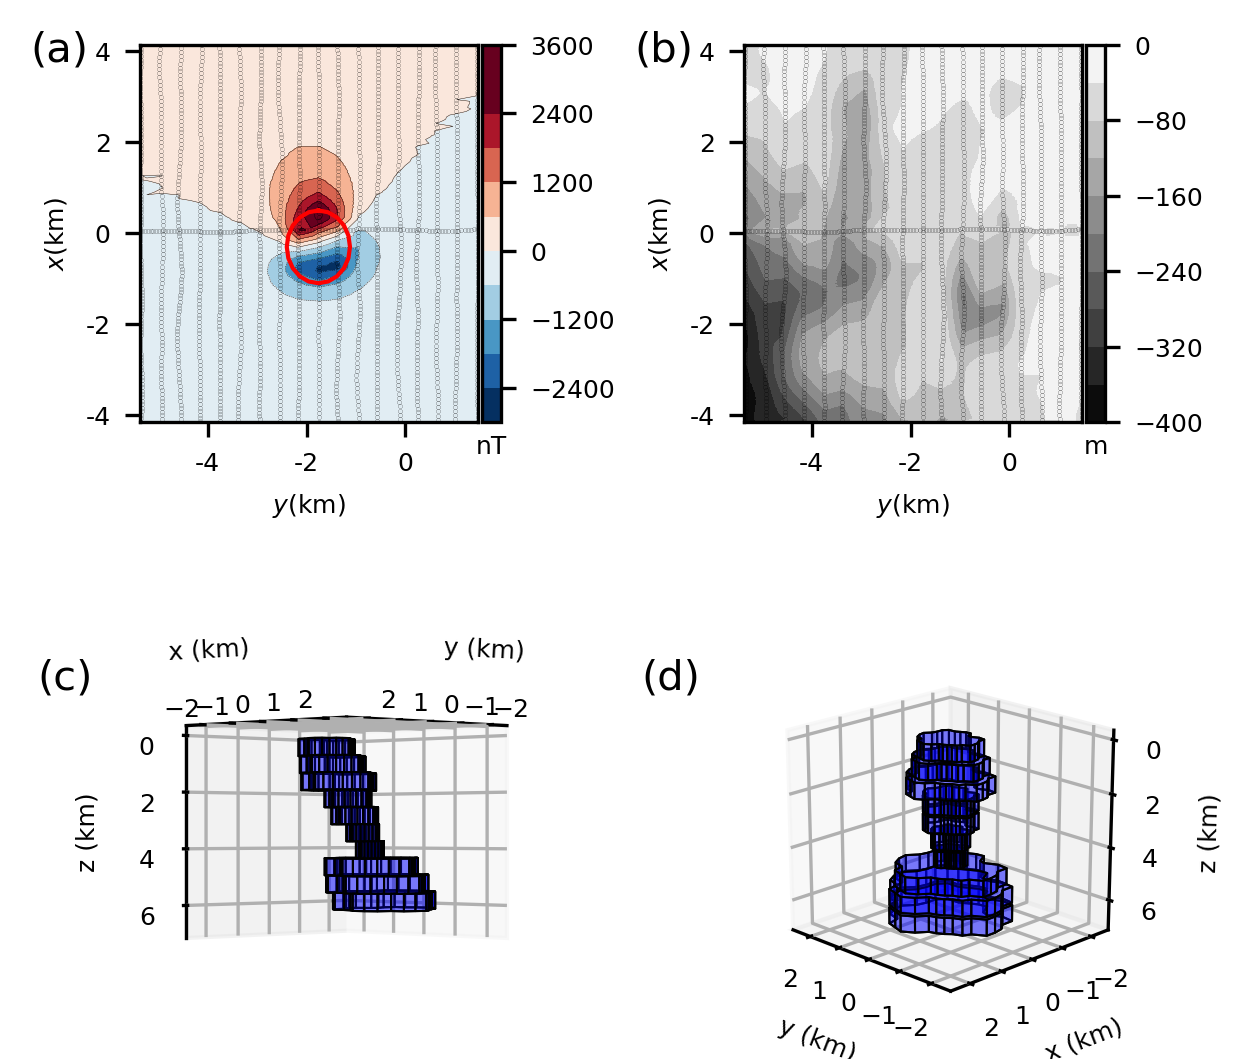
\includegraphics[width=\textwidth]{complex_model_data.png}
	\caption{Modelo da fonte alvo. (a) Anomalia de campo total contaminada com ruído produzida pela fonte alvo (prismas azuis mostrados nos painéis c e d). Os pontos pretos representam os pontos de observação. O círculo vermelho representa a projeção horizontal da aproximação inicial $\hat{\mathbf{p}}_{(0)}$ (prismas vermelhos nas Figuras
		\ref{fig:target_l2_result}c e \ref{fig:target_l1_result}c). (b) Coordenadas verticais dos pontos de observação que simulam um levantamento aéreo.
		(c) e (d) Visualizações em perspectiva do modelo da fonte alvo representado pelos prismas azuis.
	}
	\label{fig:target_model}
\end{figure}
\pagebreak
\section{Resultados sem fontes interferentes}
\label{sec:target_source_without_interference}


A Figura \ref{fig:target_model_rtp} mostra a anomalia RTP obtida da anomalia de campo total contaminada com ruído (Figura \ref{fig:target_model}a) e 
a projeção horizontal das aproximações iniciais $\hat{\mathbf{p}}_{(0)}$ 
usadas nas sucessivas inversões (Figuras \ref{fig:target_l2_result} e 
\ref{fig:target_l1_result}).
A Figura \ref{fig:target_l2_result}a mostra que a melhor solução L2 foi obtida através dos valores verdadeiros de profundidade do topo $z_{0}$ e intensidade de magnetização total $m_{0}$. Essa solução L2 produz um ótimo ajuste dos dados (Figura \ref{fig:target_l2_result}b), possui uma profundidade da base em $6641.8$ m e também recupera a geometria do corpo verdadeiro (Figura \ref{fig:target_l2_result}d).
A Figura \ref{fig:target_l1_result} mostra um resultado similarmente ótimo produzido pela melhor solução L1, que tem profundidade da base $6156.5$ m.
O aspecto mais interessante das solução L2 e L1 obtidos neste teste é que eles recuperam não só as feições principais da fonte mas também seu mergulho e a variação de sua forma ao longo da profundidade.
Todas as soluções L2 e L1 produzidas neste teste foram obtidas usando o seguinte conjunto de pesos normalizados $\tilde{\alpha}_{\ell}$ (Equação \ref{eq:alphas}): 
$\tilde{\alpha}_{1} = 10^{-5}$, $\tilde{\alpha}_{2} = 10^{-4}$, 
$\tilde{\alpha}_{3} = 10^{-4}$, $\tilde{\alpha}_{4} = 10^{-8}$, e 
$\tilde{\alpha}_{5} = 10^{-5}$. 
É importante notar que, devido à ausência de fontes interferentes neste teste, não há diferenças práticas entre as soluções L2 e L1 obtidas pelo método aqui proposto.

\begin{figure}[!htb]
	\centering
	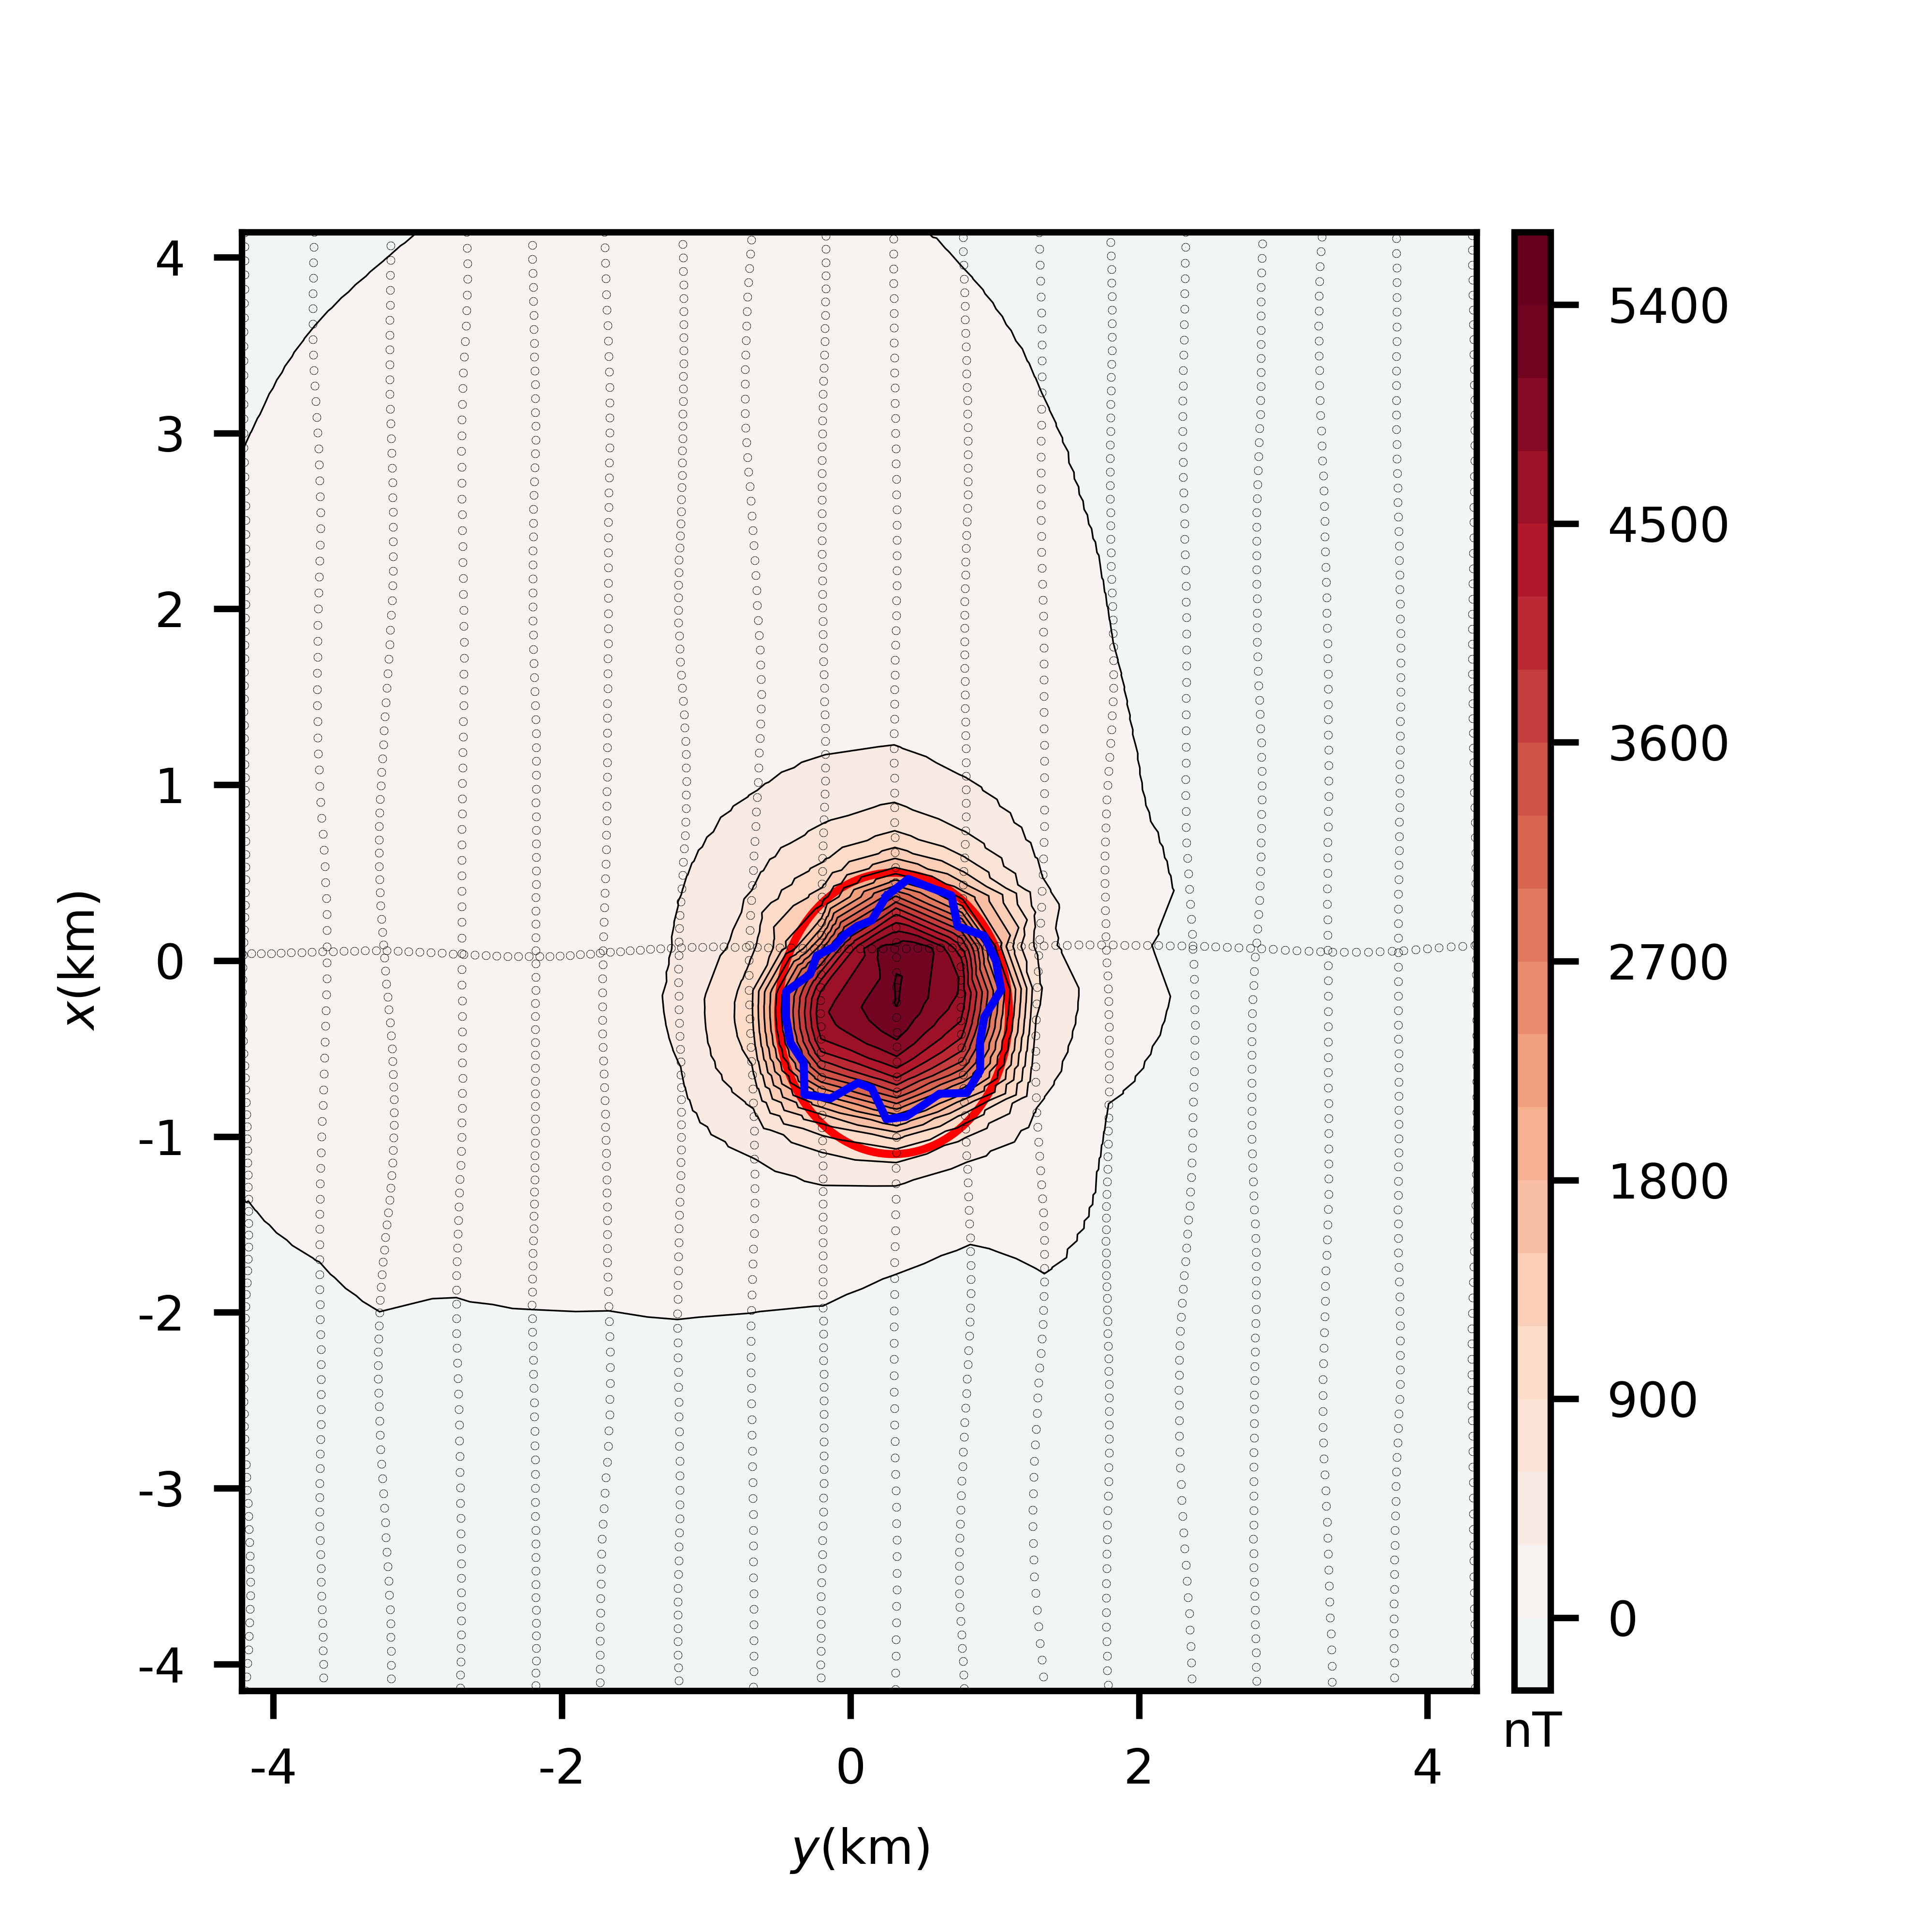
\includegraphics[width=0.5\textwidth]{complex_rtp.png}
	\caption{Anomalia RTP estimada produzida pela fonte alvo. 
		A anomalia RTP mostra valores predominantemente positivos logo acima da fonte alvo. Os pontos pretos representam os pontos de observação. As linhas azuis e vermelhas correspondem, respectivamente, às projeções horizontais da porção mais rasa da fonte alvo e da aproximação inicial utilizada nas inversões subsequentes (prismas vermelhos nas Figuras \ref{fig:target_l2_result}c e 
		\ref{fig:target_l1_result}c).
	}
	\label{fig:target_model_rtp}
\end{figure}

\pagebreak

\begin{figure}[!htb]
	\centering
	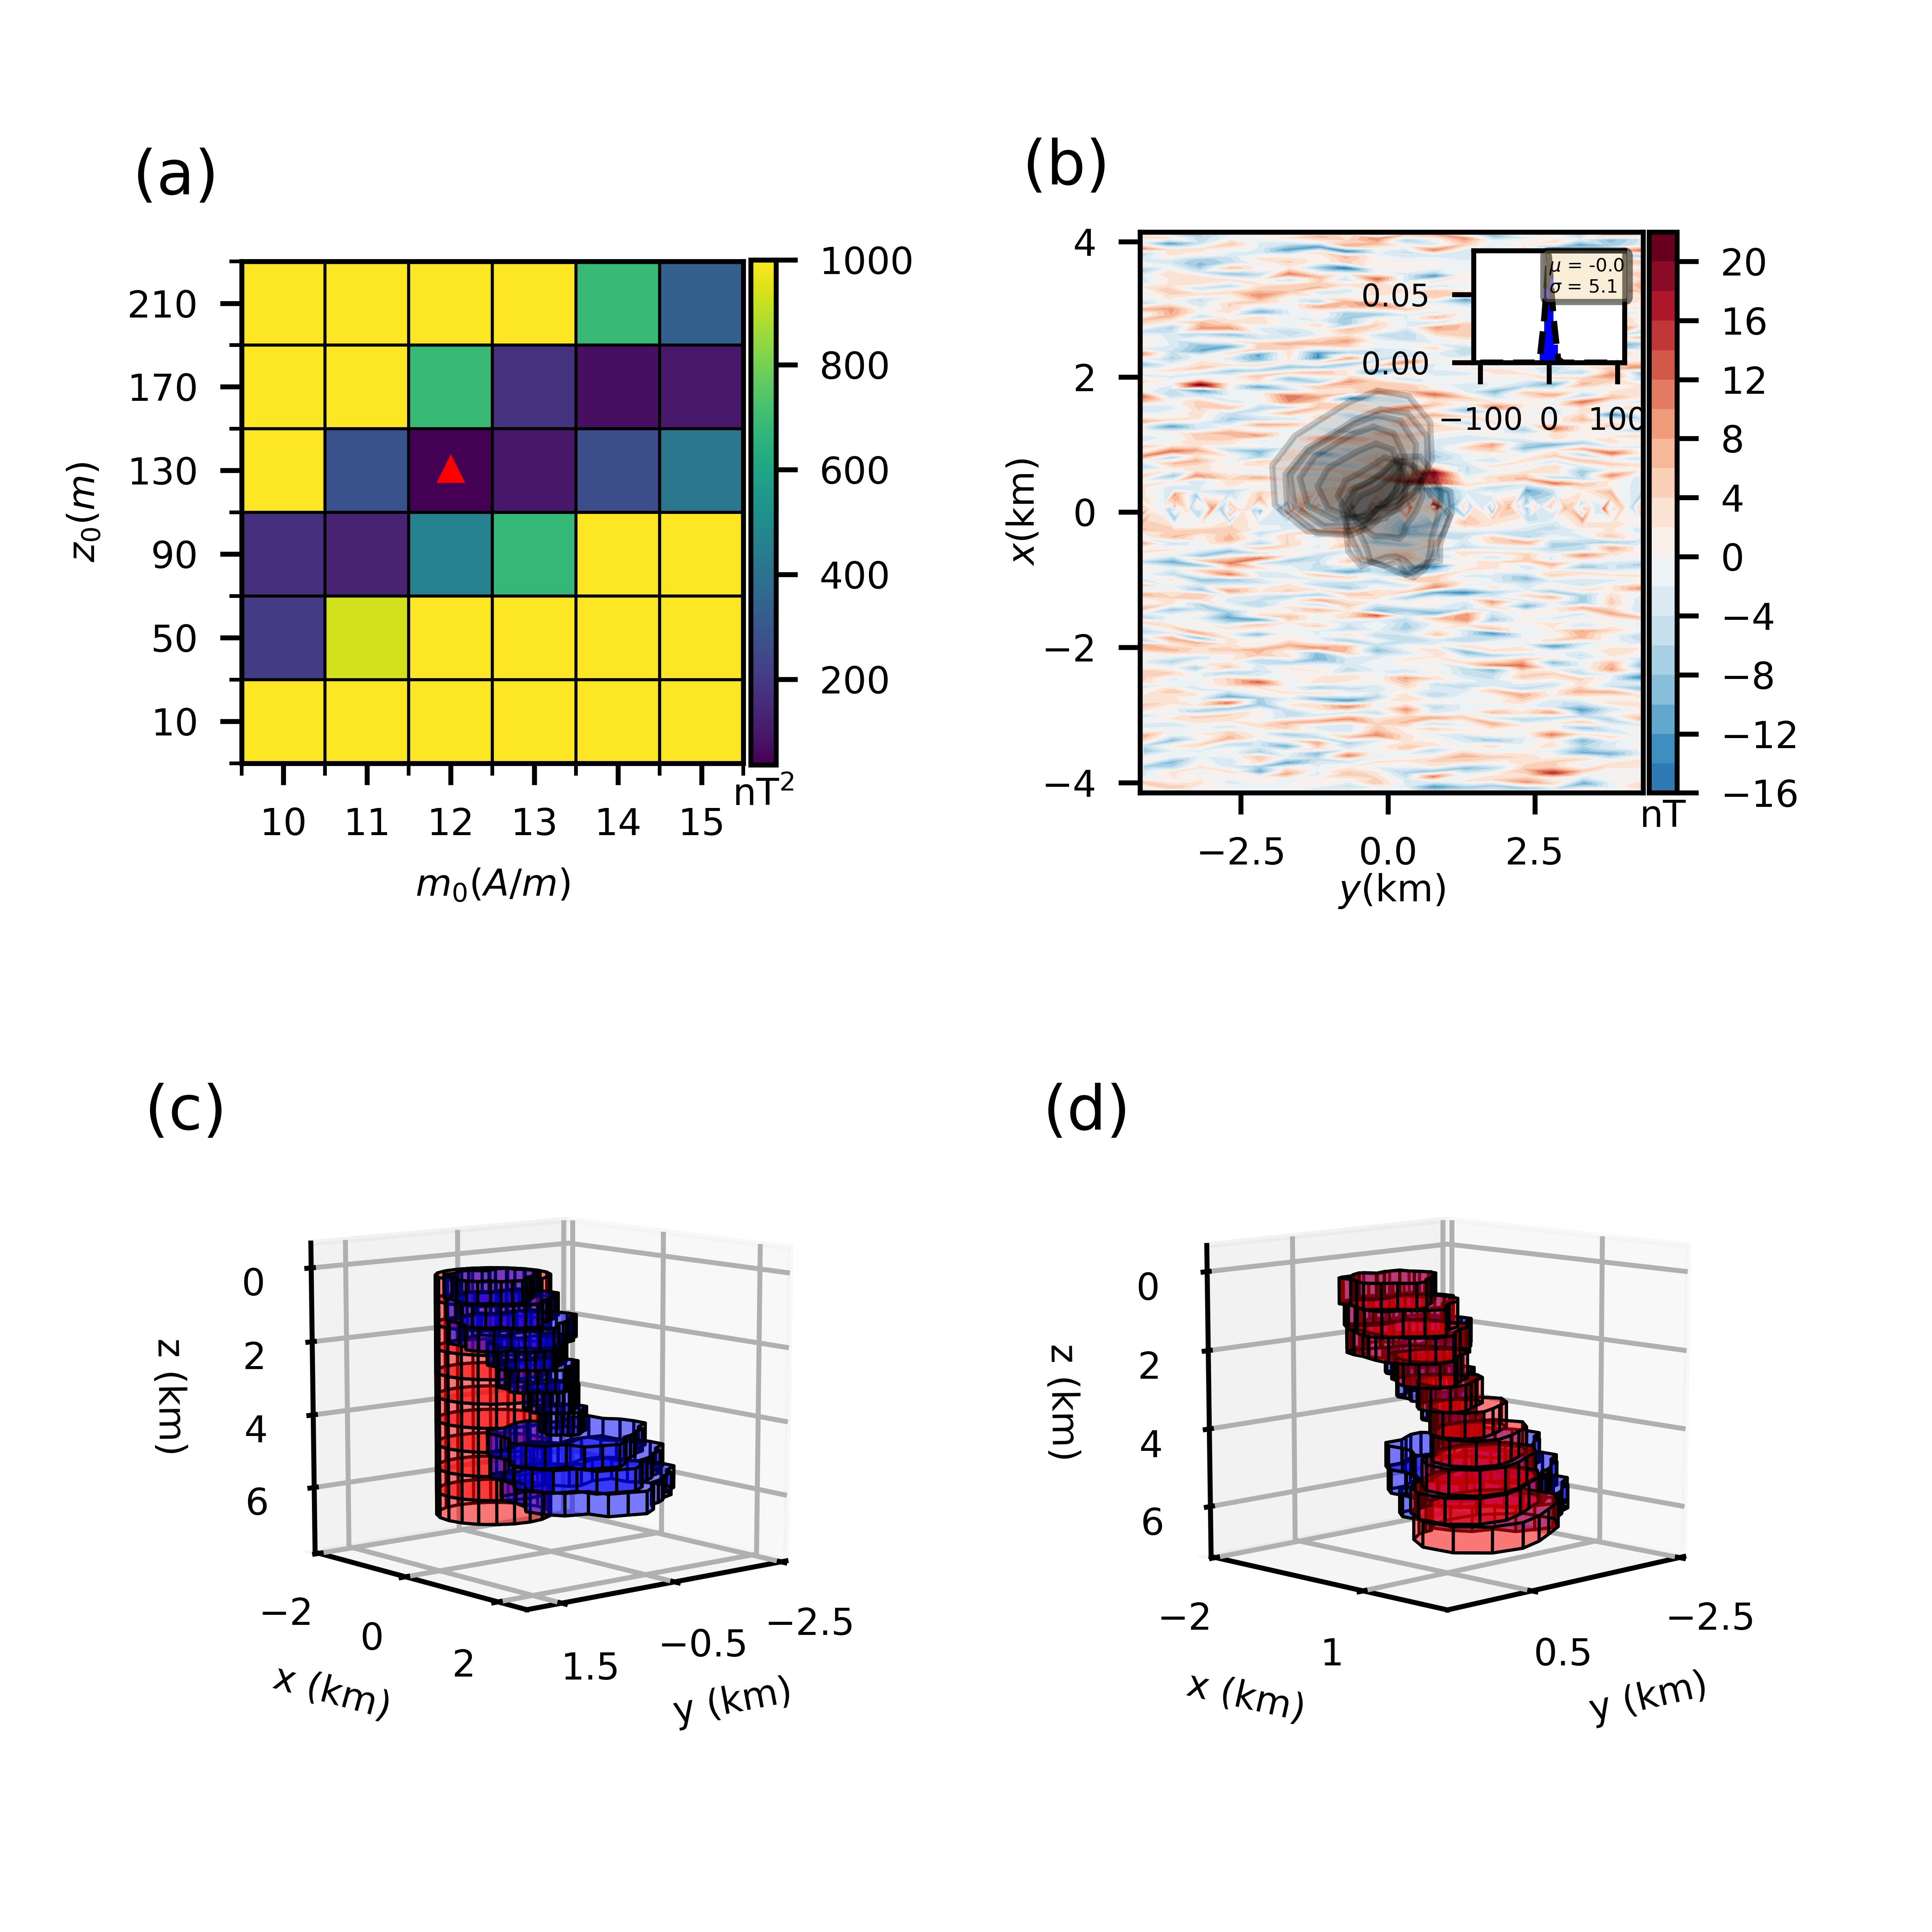
\includegraphics[width=\textwidth]{complex-l2-solution.png}
	\caption{Soluções L2 obtidas para o modelo da fonte alvo sem interferência. 
		(a) Mapa discreto da função objetivo produzida pelos modelos da malha de varredura para valores de profundidade do topo $z_{0}$ e intensidade de magnetização total $m_{0}$. 
		O triângulo vermelho representa os valores verdadeiros para $m_{0}$ e $z_{0}$, assim como os valores que definem a melhor solução L2.
		(b) Resíduos entre os dados contaminados com ruído (Fig. \ref{fig:target_model}a) 
		e os dados preditos (não mostrados) produzidos pela melhor solução L2 (prismas vermelhos no painel d). 
		O histograma dos resíduos inserido em (b) mostra a curva Gaussiana ajustada (curva tracejada).
		Os polígonos cinzas representam as projeções horizontais de todos os prismas que compõe a melhor solução. 
		(c) e (d) Visualização em perspectiva da aproximação inicial (prismas vermelhos) e 
		a melhor solução (prismas vermelhos), respectivamente. Os prismas azuis são o modelo da fonte alvo. 
	}
	\label{fig:target_l2_result}
\end{figure}

\begin{figure}[!htb]
	\centering
	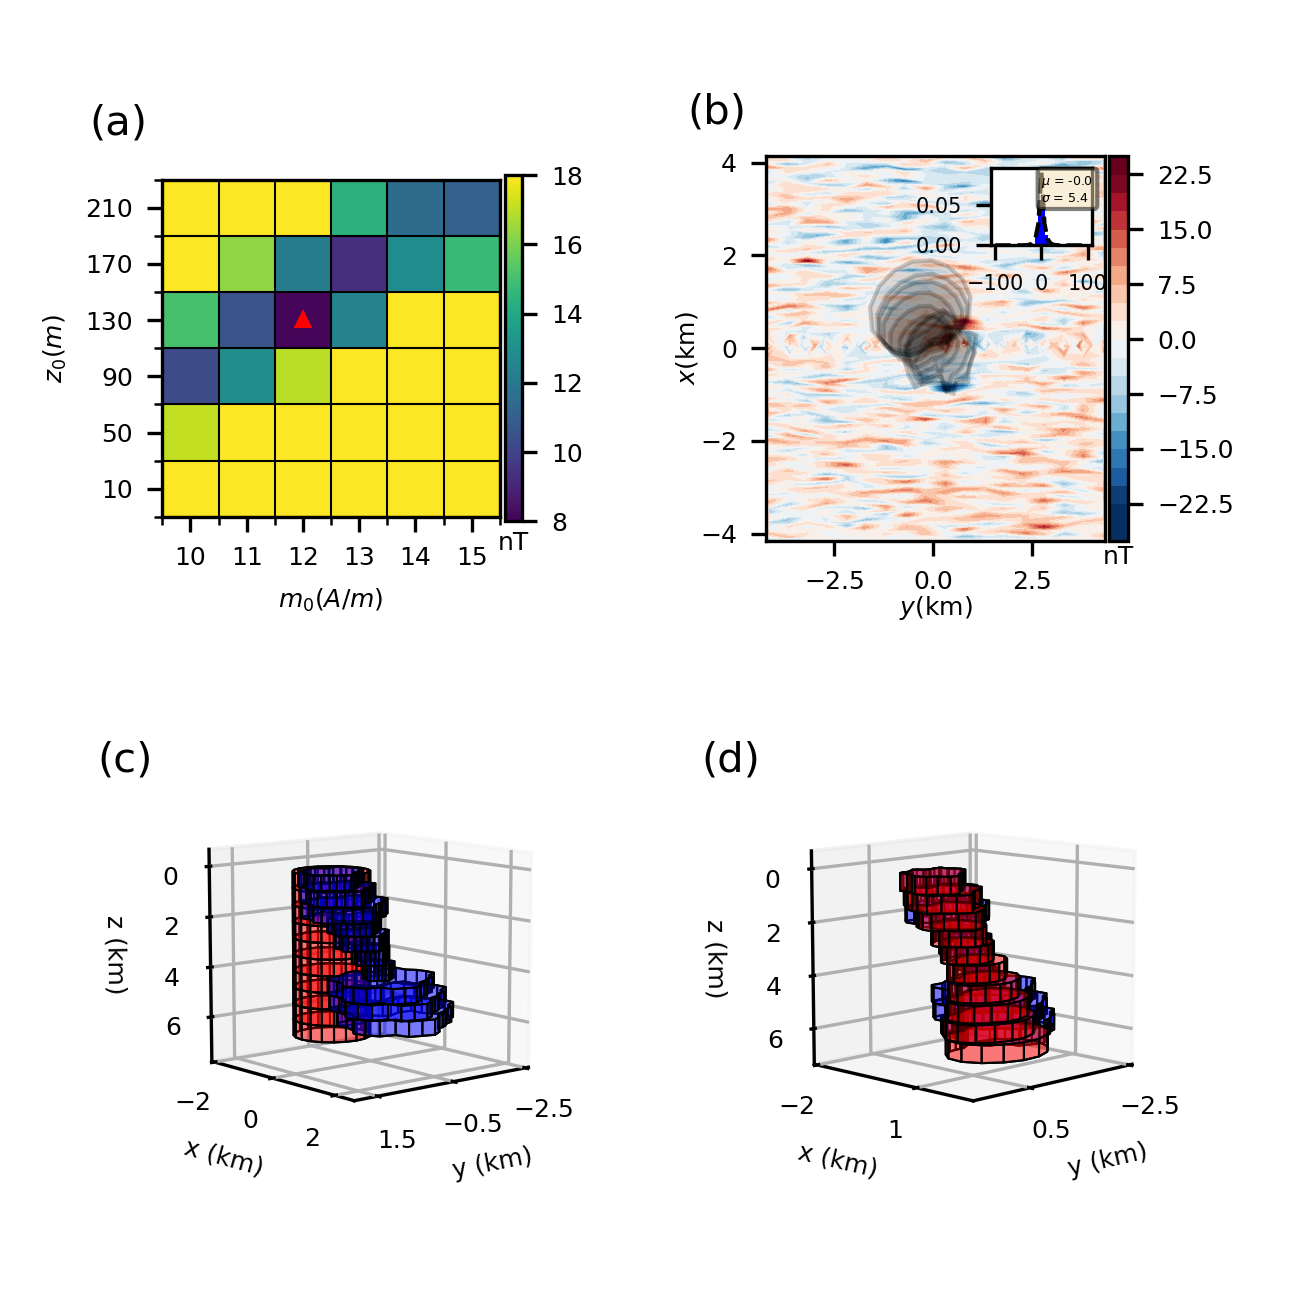
\includegraphics[width=\textwidth]{complex-l1-solution.png}
	\caption{Soluções L1 obtidas para o modelo da fonte alvo sem interferência. 
		(a) Mapa discreto da função objetivo produzida pelos modelos da malha de varredura para valores de profundidade do topo $z_{0}$ e intensidade de magnetização total $m_{0}$. 
		O triângulo vermelho representa os valores verdadeiros para $m_{0}$ e $z_{0}$, assim como os valores que definem a melhor solução L1.
		(b) Resíduos entre os dados contaminados com ruído (Fig. \ref{fig:target_model}a) 
		e os dados preditos (não mostrados) produzidos pela melhor solução L1 (prismas vermelhos no painel d). 
		O histograma dos resíduos inserido em (b) mostra a curva Laplaciana ajustada (curva tracejada).
		Os polígonos cinzas representam as projeções horizontais de todos os prismas que compõe a melhor solução. 
		(c) e (d) Visualização em perspectiva da aproximação inicial (prismas vermelhos) e 
		a melhor solução (prismas vermelhos), respectivamente. Os prismas azuis são o modelo da fonte alvo. 
	}
	\label{fig:target_l1_result}
\end{figure}

\section{Resultados com uma fonte interferente pequena}
\label{sec:target_source_with_small_interference}


O mapa da Figura \ref{fig:small_model}a representa a soma entre as anomalias de campo total produzidas pela fonte interferente pequena (Figura \ref{fig:small_model}b), cuja forma é exibida nas Figuras \ref{fig:small_model}c e \ref{fig:small_model}d, e aquela produzida pela fonte alvo simulada (Figura \ref{fig:target_model}a). 
A fonte interferente possui profundidade do topo em $0$ m, profundidade da base em $70$ m, 
centro em $(x, y) = (-250, 250)$, logo acima a parte mais rasa da fonte alvo, e o mesmo vetor magnetização total da fonte alvo.
Embora a nova anomalia RTP produzida com a fonte interferente (Figura 
\ref{fig:small_model_rtp}) tem uma amplitude maior que a produzida pela fonte alvo isolada (Figura \ref{fig:target_model_rtp}), a extensão horizontal da área positiva não muda substancialmente e conduz uma aproximação inicial
(Figuras \ref{fig:small_l2_result}c e \ref{fig:small_l1_result}c) igual àquela utilizada no teste anterior (Figuras \ref{fig:target_l2_result}c e 
\ref{fig:target_l1_result}c).

A Figura \ref{fig:small_l2_result} mostra as soluções L2 obtidas pela inversão da anomalia de campo total na Figura \ref{fig:small_model}a
com os seguintes pesos normalizados $\tilde{\alpha}_{\ell}$ (Equação \ref{eq:alphas}):
$\tilde{\alpha}_{1} = 10^{-5}$, $\tilde{\alpha}_{2} = 10^{-4}$, 
$\tilde{\alpha}_{3} = 10^{-4}$, $\tilde{\alpha}_{4} = 10^{-8}$, e 
$\tilde{\alpha}_{5} = 10^{-5}$.
A Figura \ref{fig:small_l2_result}a mostra que a melhor solução L2 possui profundidade do topo $z_{0}$ igual à verdadeira, porém possui uma intensidade de magnetização total $m_{0}$ superestimada. Por esse motivo, sua profundidade máxima 
($3046.8$ m) é muito distante da verdadeira ($6130$ m).
Essa solução produz valores de resíduos altos logo acima a fonte interferente  
(Figura \ref{fig:small_l2_result}b), mas esses resíduos diferem consideravelmente da anomalia de campo total produzida pela fonte interferente (Figura \ref{fig:small_model}b).
Isso significa que, nesse caso, a inversão não foi capaz de ignorar o efeito causado pela fonte interferente.
Além disso, a Figura \ref{fig:small_l2_result}d mostra que a melhor solução L2 não recupera a forma da fonte alvo.

A Figura \ref{fig:small_l1_result} mostra as soluções L1 obtidas pela inversão da anomalia de campo total exibida na Figura \ref{fig:small_model}a
com os mesmos pesos normalizados $\tilde{\alpha}_{\ell}$ (Equação \ref{eq:alphas})
utilizados para as soluções L2 (Figura \ref{fig:small_l2_result}).
Comparada à solução L2 mostrada na Figura \ref{fig:small_l2_result}, a melhor solução L1 apresenta uma intensidade de magnetização total menos superestimada (Figura 
\ref{fig:small_l1_result}a) e profundidade da base ($5176.4$ m) próxima à verdadeira ($6130$ m). Essa solução produz valores de resíduos (Figura \ref{fig:small_l1_result}b) 
próximos à anomalia de campo total produzida pela fonte interferente (Figura 
\ref{fig:small_model}b). 
Isso significa que, nesse caso, a performance do método foi mais eficaz em filtrar a anomalia de campo total interferente (Figura \ref{fig:small_model}b).
Como consequência, a solução L1 (Figura \ref{fig:small_l1_result}d) foi muito menos afetada pela fonte interferente e recuperou satisfatoriamente a forma da fonte alvo. 
Este teste numérico mostra que a solução L1 é superior à solução L2 mesmo que a fonte interferente seja muito localizada e menor do que a fonte alvo.

\section{Resultados com uma fonte interferente grande}
\label{sec:target_source_with_large_interference}

O mapa da Figura \ref{fig:thick_model}a representa a soma entre as anomalias de campo total produzidas pela fonte interferente pequena (Figura \ref{fig:thick_model}b), cuja forma é exibida nas Figuras \ref{fig:thick_model}c e \ref{fig:thick_model}d, e aquela produzida pela fonte alvo simulada (Figura \ref{fig:target_model}a).
A fonte interferente possui profundidade do topo em $0$ m, profundidade da base em $500$ m, 
centro em $(x, y) = (500, 1500)$, ao lado do topo da fonte alvo, e o mesmo vetor magnetização total da fonte alvo.
Neste caso, a fonte interferente estende consideravelmente a área positiva da anomalia RTP (Figura \ref{fig:thick_model_rtp}) em comparação com a da fonte alvo isolada (Figura \ref{fig:target_model_rtp}). Entretanto, ainda é possível identificar os limites laterais da fonte alvo e gerar a mesma aproximação inicial usada nos testes anteriores.


A Figura \ref{fig:thick_l2_result} mostra as soluções L2 obtidas pela inversão da anomalia de campo total na Figura \ref{fig:thick_model}a
com os seguintes pesos normalizados $\tilde{\alpha}_{\ell}$ (Equação \ref{eq:alphas}):
$\tilde{\alpha}_{1} = 10^{-4}$, $\tilde{\alpha}_{2} = 10^{-5}$, 
$\tilde{\alpha}_{3} = 10^{-4}$, $\tilde{\alpha}_{4} = 10^{-7}$, e 
$\tilde{\alpha}_{5} = 10^{-7}$.
Como podemos ver, a melhor solução L2 não recupera os valores de profundidade do topo $z_{0}$ e nem de intensidade de magnetização total $m_{0}$, assim como não recuperou a forma da fonte alvo.
A estimativa da profundidade da base ($2010.1$ m) é muito distante da verdadeira ($6130$ m).
Comparado ao valor verdadeiro, a profundidade do topo estimada $z_{0}$ está deslocada em direção à da fonte interferente.
Neste caso, a fonte interferente induz severamente ao erro a geometria do corpo estimado (Figura \ref{fig:thick_l2_result}d).

A Figura \ref{fig:thick_l1_result} mostra as soluções L1 obtidas pela inversão da anomalia de campo total mostrada na Figura \ref{fig:thick_model}a
com os seguintes pesos normalizados $\tilde{\alpha}_{\ell}$ (Equação \ref{eq:alphas}):
$\tilde{\alpha}_{1} = 10^{-4}$, $\tilde{\alpha}_{2} = 10^{-5}$, 
$\tilde{\alpha}_{3} = 10^{-4}$, $\tilde{\alpha}_{4} = 10^{-7}$, e 
$\tilde{\alpha}_{5} = 10^{-7}$.
A melhor solução L1 (Figura \ref{fig:thick_l1_result}) filtra parcialmente a anomalia de campo total interferente (Figura \ref{fig:thick_model}b) e recupera as principais feições da fonte alvo sintética, assim como a profundidade do topo $z_{0}$ e a intensidade de magnetização total $m_{0}$ verdadeiras.
A estimativa da profundidade da base ($5840.9$ m) é muito próxima à verdadeira ($6130$ m).
Essa solução é inferior à mostrada no teste anterior (Figura \ref{fig:small_l1_result})
em filtrar a anomalia de campo total interferente e também em recuperar a forma da fonte alvo. 
Apesar disso, ela é significativamente superior à melhor solução L2 (Figura \ref{fig:thick_l2_result}) obtida pela inversão do mesmo dado, uma vez que é muito menos afetada pela presença de uma grande fonte interferente.

\begin{figure}[!htb]
	\centering
	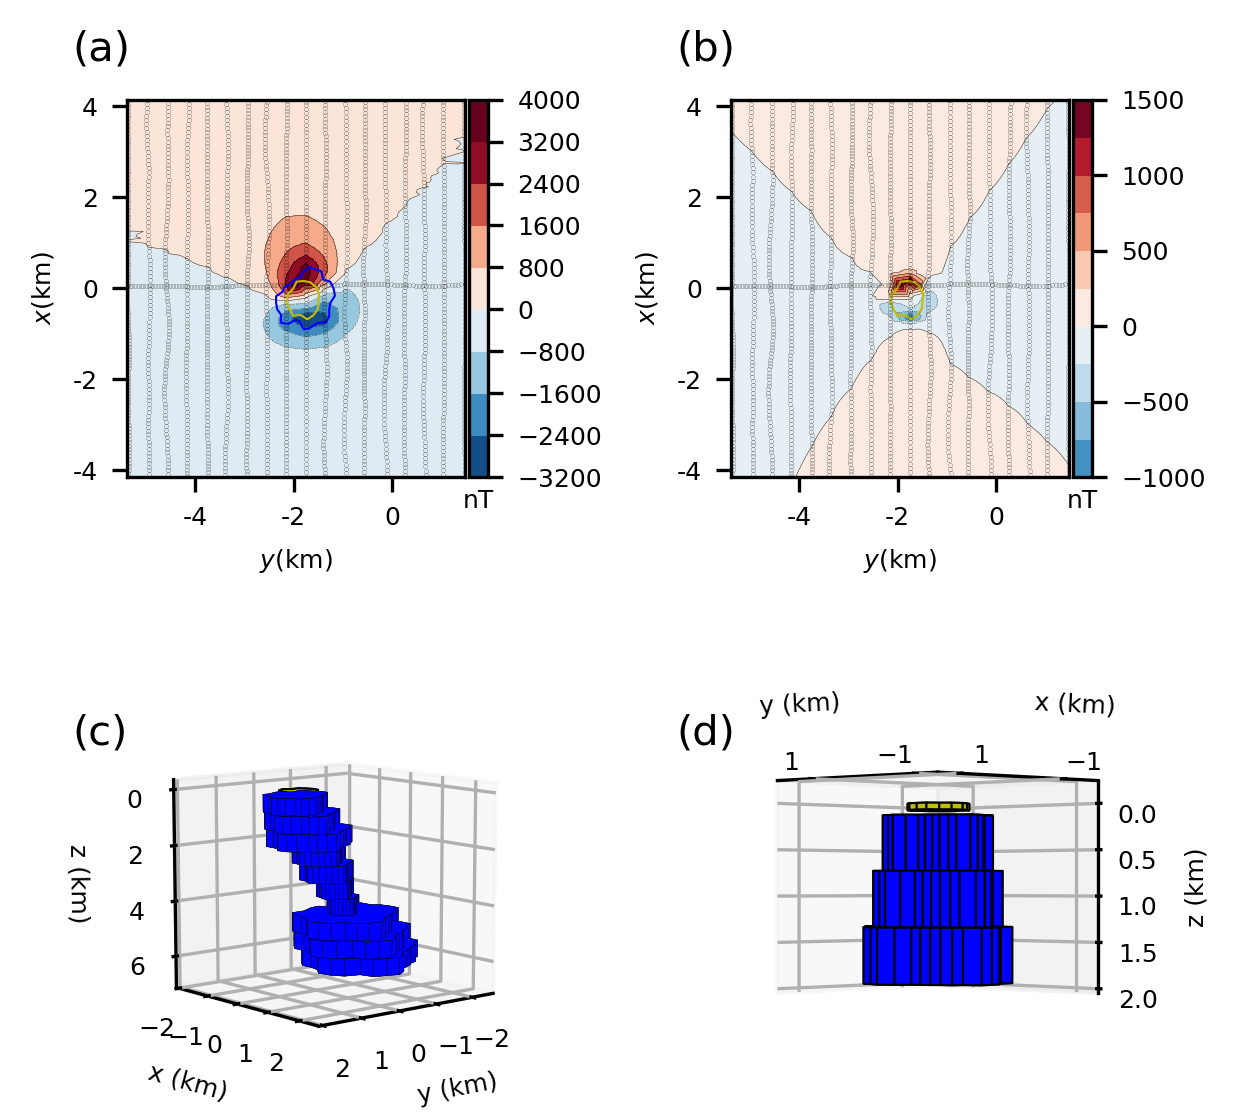
\includegraphics[width=\textwidth]{small_model_data.png}
	\caption{Modelo da fonte alvo com uma fonte interferente pequena.
		(a) Anomalia de campo total produzida pelas fontes alvo e interferente
		(prismas azuis e amarelos nos painéis c e d). Os pontos pretos representam os pontos de observação. Os polígonos azul e amarelo são as projeções horizontais das fontes alvo e interferente, respectivamente.
		(b) A anomalia de campo total produzida pela fonte interferente. 
		(c) Visualização em perspectiva da fonte alvo (prismas azuis) e da fonte interferente (prisma amarelo). 
		(d) Visualização em perspectiva aproximada das fontes alvo (prismas azuis) e interferente (prisma amarelo).
	}
	\label{fig:small_model}
\end{figure}

\begin{figure}[!htb]
	\centering
	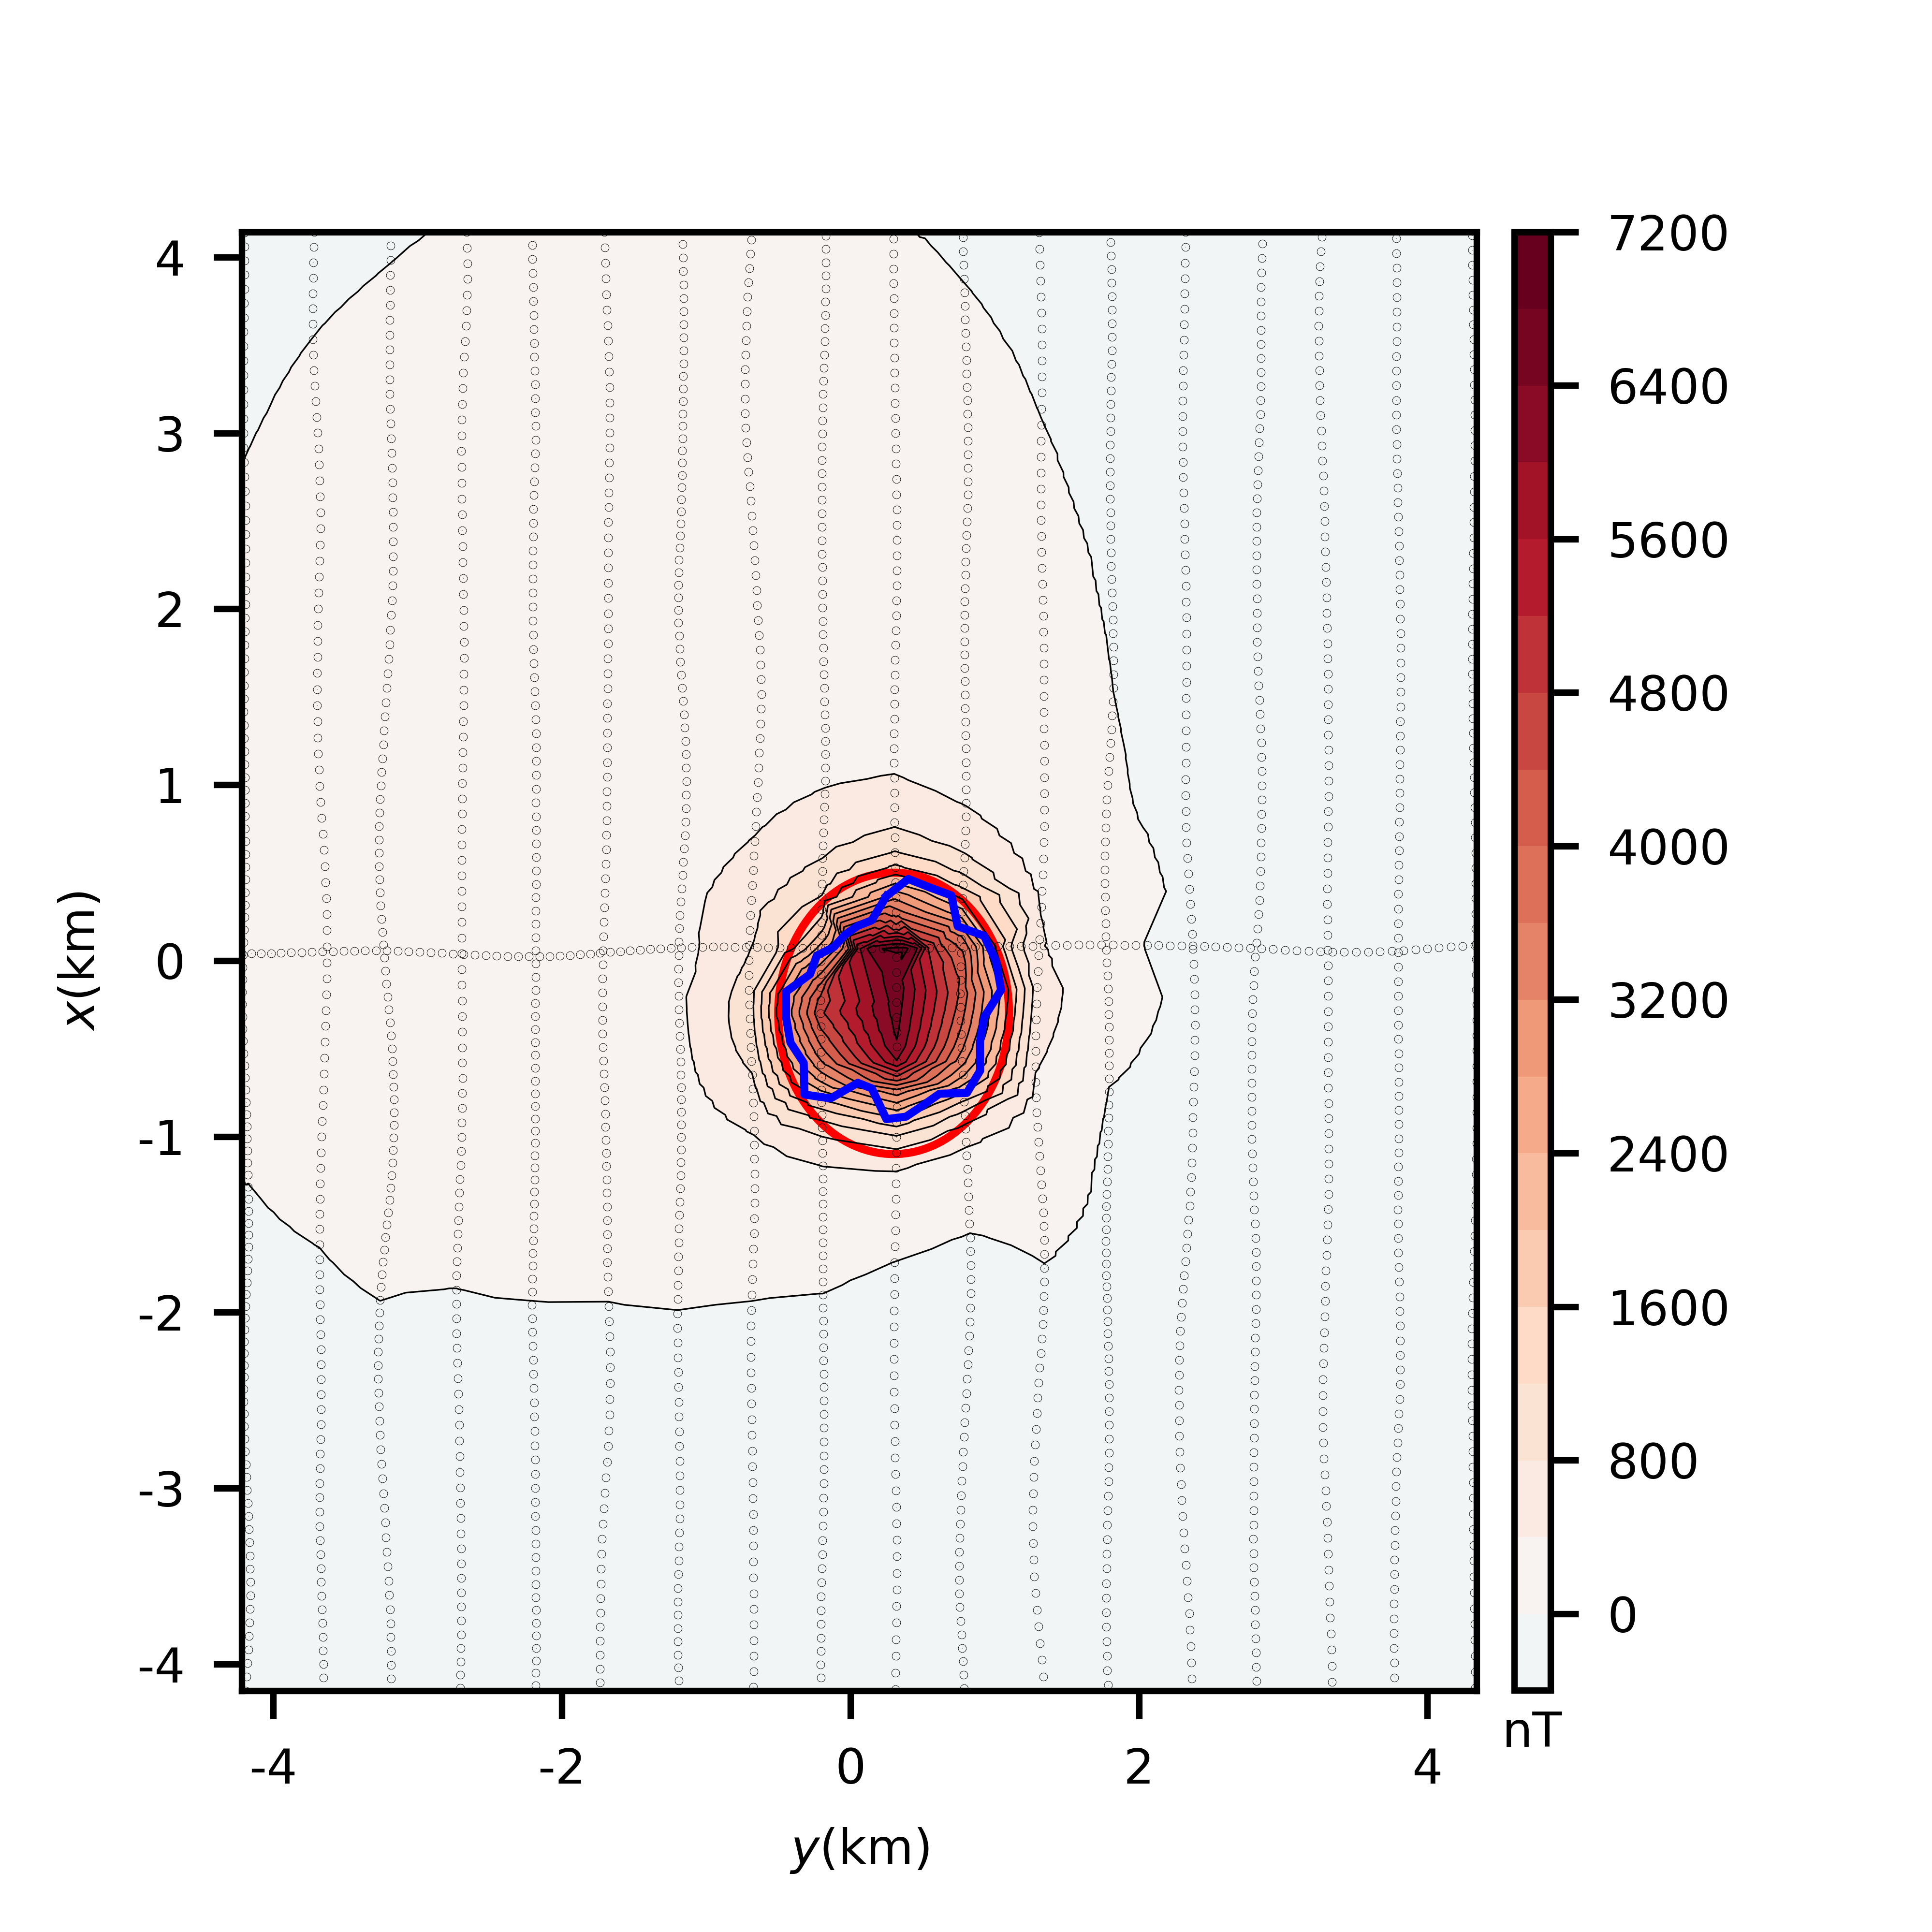
\includegraphics[width=0.5\textwidth]{small_rtp.png}
	\caption{Anomalia RTP estimada produzida pela fonte alvo com uma fonte interferente pequena. 
		A anomalia RTP mostra valores predominantemente positivos logo acima da fonte alvo. Os pontos pretos representam os pontos de observação. As linhas azuis e vermelhas correspondem, respectivamente, às projeções horizontais da porção mais rasa da fonte alvo e da aproximação inicial utilizada nas inversões subsequentes (prismas vermelhos nas Figuras \ref{fig:small_l2_result}c e 
		\ref{fig:small_l1_result}c).
	}
	\label{fig:small_model_rtp}
\end{figure}

\begin{figure}[!htb]
	\centering
	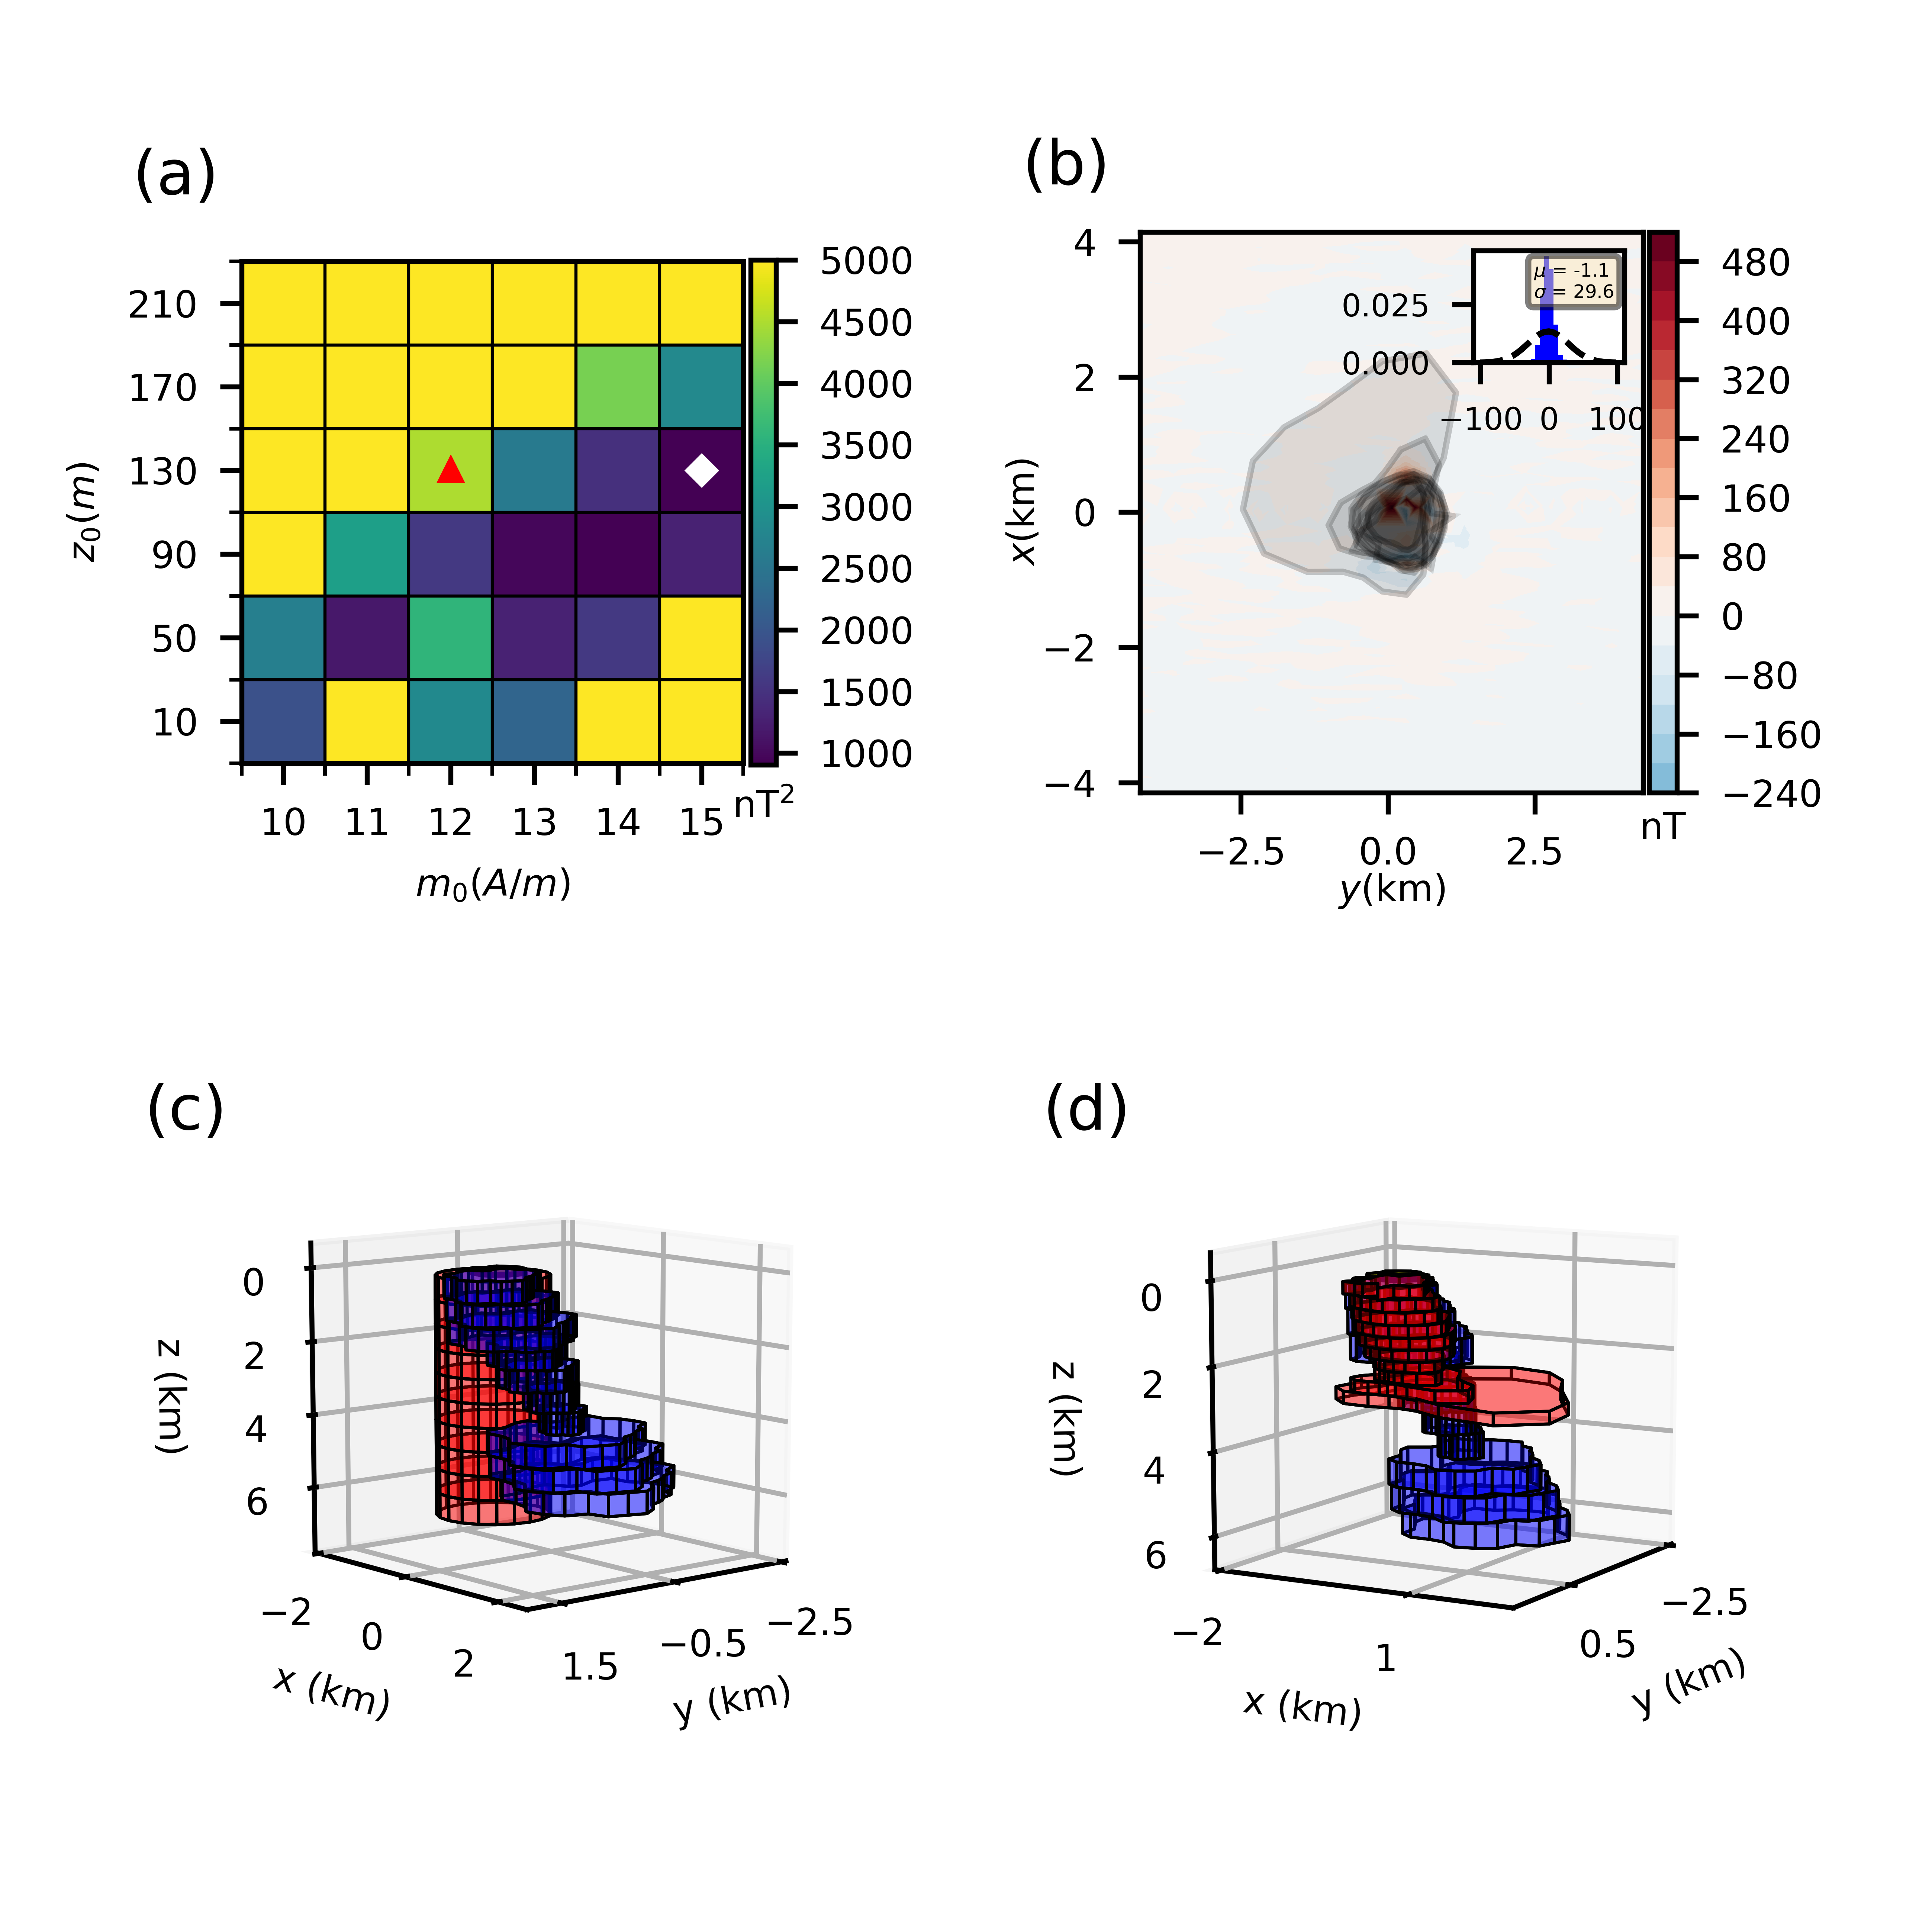
\includegraphics[width=\textwidth]{small-l2-solution.png}
	\caption{Soluções L2 obtidas para o modelo da fonte alvo com uma fonte interferente pequena. 
		(a) Mapa discreto da função objetivo produzida pelos modelos da malha de varredura para valores de profundidade do topo $z_{0}$ e intensidade de magnetização total $m_{0}$. 
		Os valores verdadeiros de $m_{0}$ e $z_{0})$ e aqueles que definem a melhor solução L2 são representados pelo triângulo vermelho e pelo losango branco, respectivamente.
		(b) Resíduos entre os dados contaminados com ruído (Fig. \ref{fig:target_model}a) 
		e os dados preditos (não mostrados) produzidos pela melhor solução L2 (prismas vermelhos no painel d). 
		O histograma dos resíduos inserido em (b) mostra a curva Gaussiana ajustada (curva tracejada).
		Os polígonos cinzas representam as projeções horizontais de todos os prismas que compõe a melhor solução. 
		(c) e (d) Visualização em perspectiva da aproximação inicial (prismas vermelhos) e 
		a melhor solução (prismas vermelhos), respectivamente. Os prismas azuis são o modelo da fonte alvo.
	}
	\label{fig:small_l2_result}
\end{figure}

\begin{figure}[!htb]
	\centering
	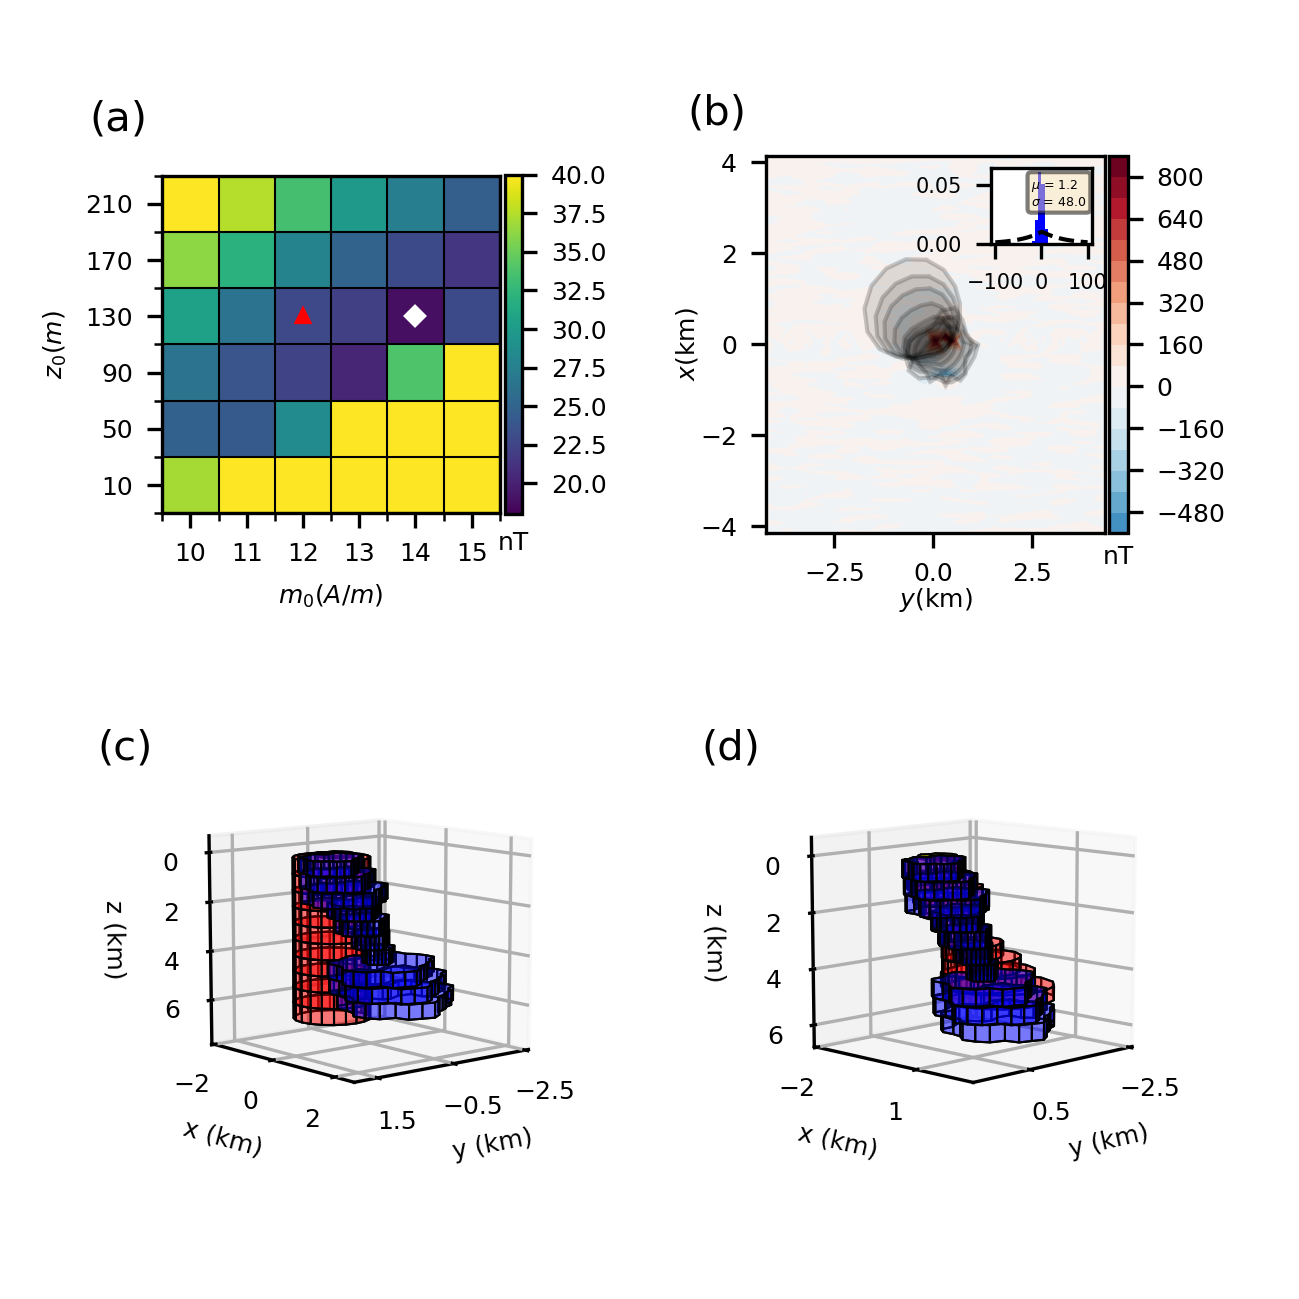
\includegraphics[width=\textwidth]{small-l1-solution.png}
	\caption{Soluções L1 obtidas para o modelo da fonte alvo com uma fonte interferente pequena. 
		(a) Mapa discreto da função objetivo produzida pelos modelos da malha de varredura para valores de profundidade do topo $z_{0}$ e intensidade de magnetização total $m_{0}$. 
		Os valores verdadeiros de $m_{0}$ e $z_{0})$ e aqueles que definem a melhor solução L1 são representados pelo triângulo vermelho e pelo losango branco, respectivamente.
		(b) Resíduos entre os dados contaminados com ruído (Fig. \ref{fig:target_model}a) 
		e os dados preditos (não mostrados) produzidos pela melhor solução L1 (prismas vermelhos no painel d). 
		O histograma dos resíduos inserido em (b) mostra a curva Gaussiana ajustada (curva tracejada).
		Os polígonos cinzas representam as projeções horizontais de todos os prismas que compõe a melhor solução. 
		(c) e (d) Visualização em perspectiva da aproximação inicial (prismas vermelhos) e 
		a melhor solução (prismas vermelhos), respectivamente. Os prismas azuis são o modelo da fonte alvo. 
	}
	\label{fig:small_l1_result}
\end{figure}

\begin{figure}[!htb]
	\centering
	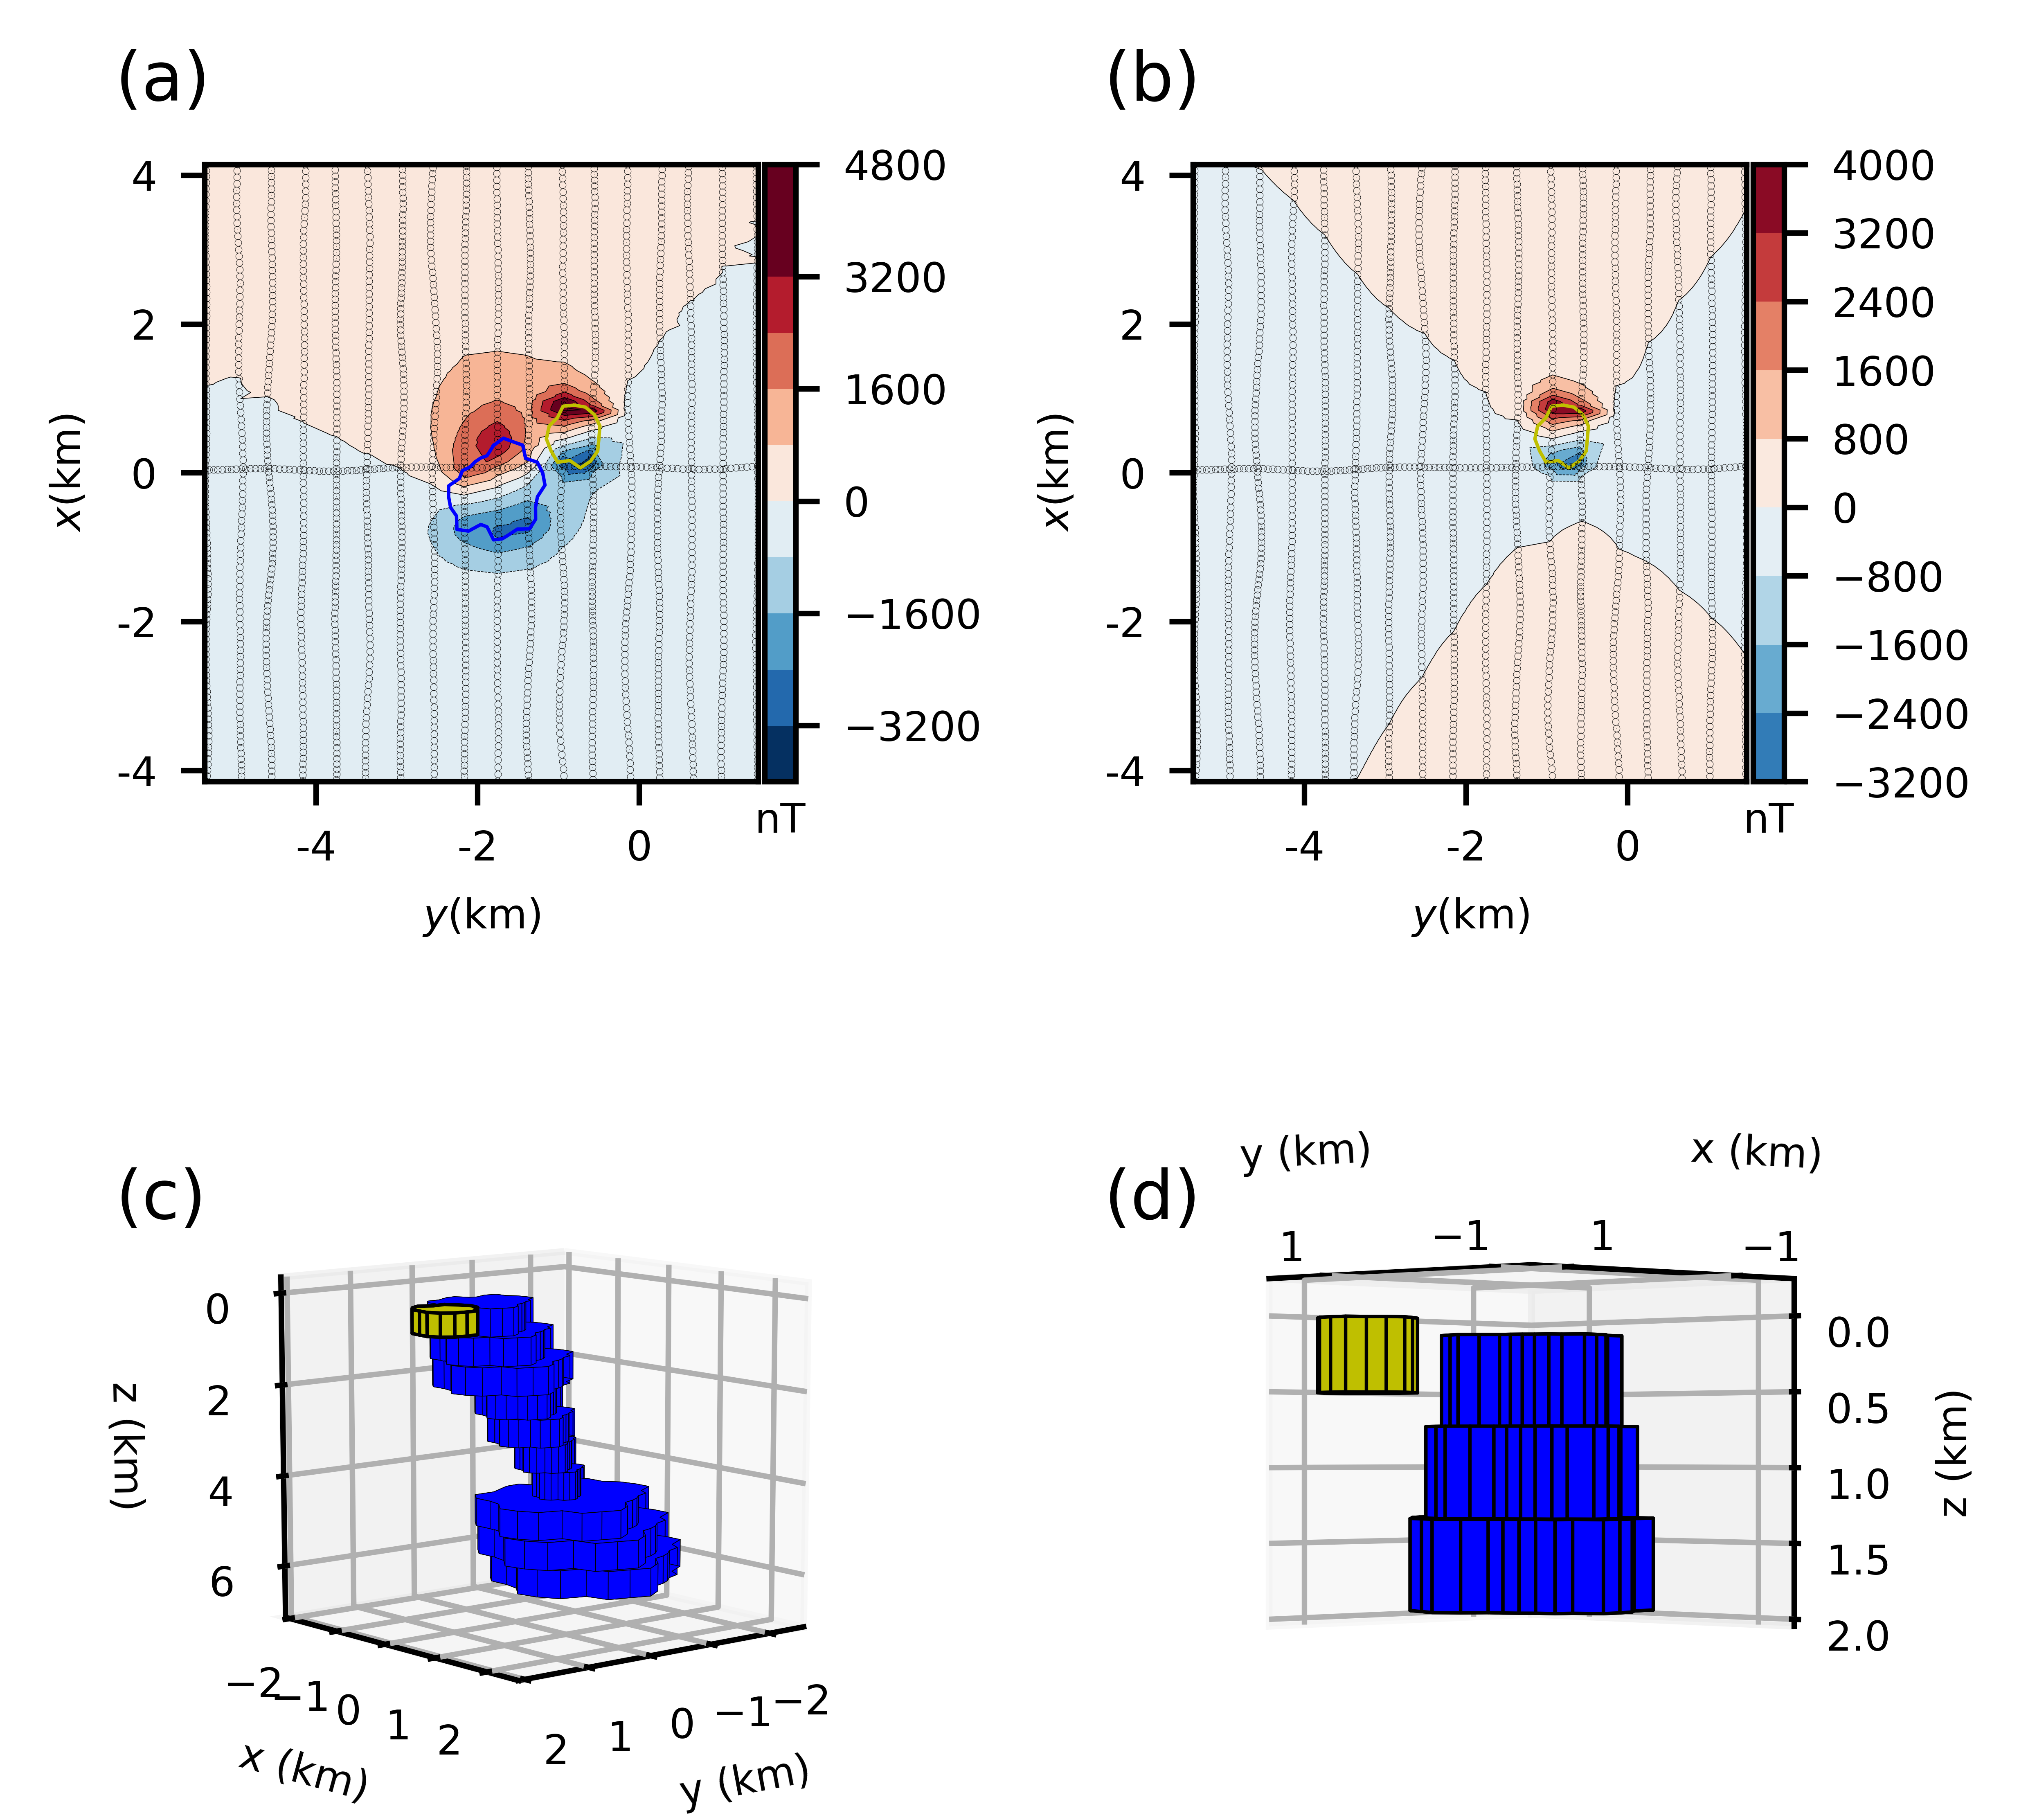
\includegraphics[width=\textwidth]{thick_model_data.png}
	\caption{Modelo da fonte alvo com uma fonte interferente grande.
		(a) Anomalia de campo total produzida pelas fontes alvo e interferente
		(prismas azuis e amarelos nos painéis c e d). Os pontos pretos representam os pontos de observação. Os polígonos azul e amarelo são as projeções horizontais das fontes alvo e interferente, respectivamente.
		(b) A anomalia de campo total produzida pela fonte interferente. 
		(c) Visualização em perspectiva da fonte alvo (prismas azuis) e da fonte interferente (prisma amarelo). 
		(d) Visualização em perspectiva aproximada das fontes alvo (prismas azuis) e interferente (prisma amarelo).
	}
	\label{fig:thick_model}
\end{figure}


\begin{figure}[!htb]
	\centering
	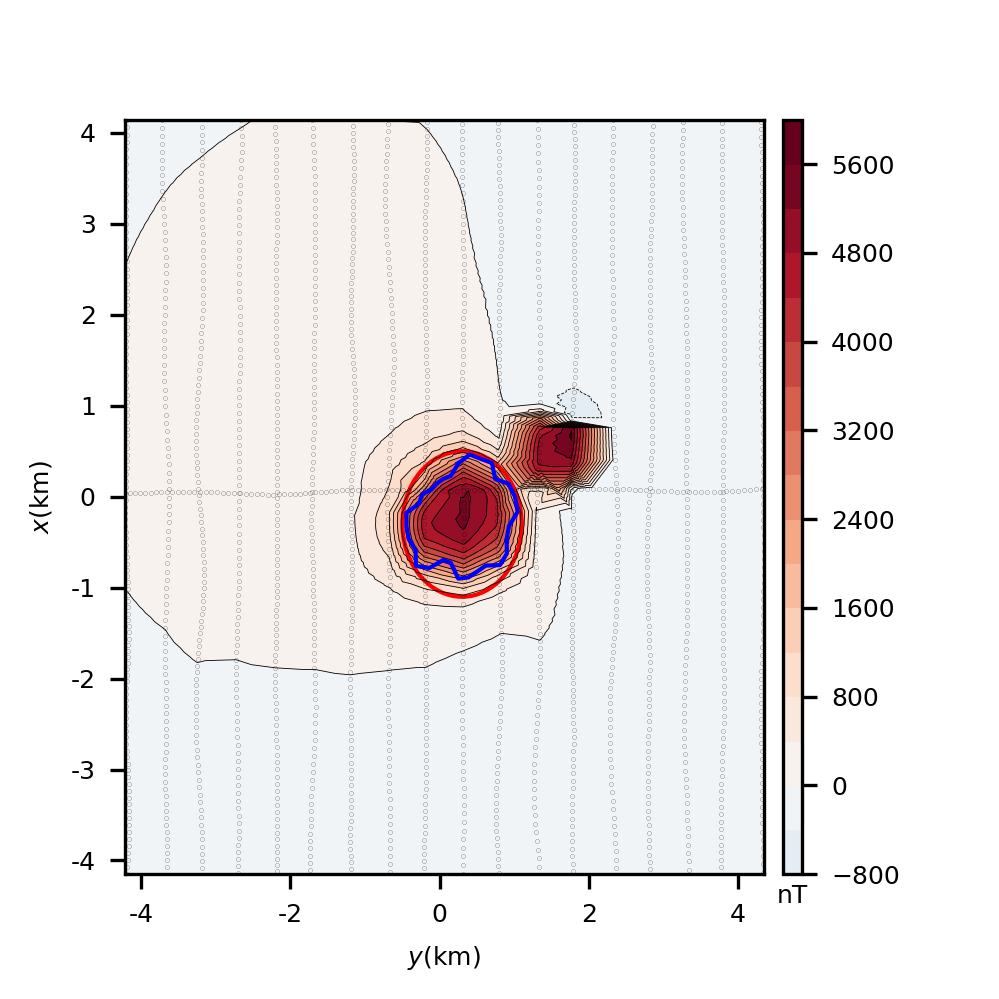
\includegraphics[width=0.5\textwidth]{thick_rtp.png}
	\caption{Anomalia RTP estimada produzida pela fonte alvo com uma fonte interferente grande. 
		A anomalia RTP mostra valores predominantemente positivos logo acima das fontes alvo e interferente. Os pontos pretos representam os pontos de observação. As linhas azuis e vermelhas correspondem, respectivamente, às projeções horizontais da porção mais rasa da fonte alvo e da aproximação inicial utilizada nas inversões subsequentes (prismas vermelhos nas Figuras \ref{fig:thick_l2_result}c e 
		\ref{fig:thick_l1_result}c).
	}
	\label{fig:thick_model_rtp}
\end{figure}

\begin{figure}[!htb]
	\centering
	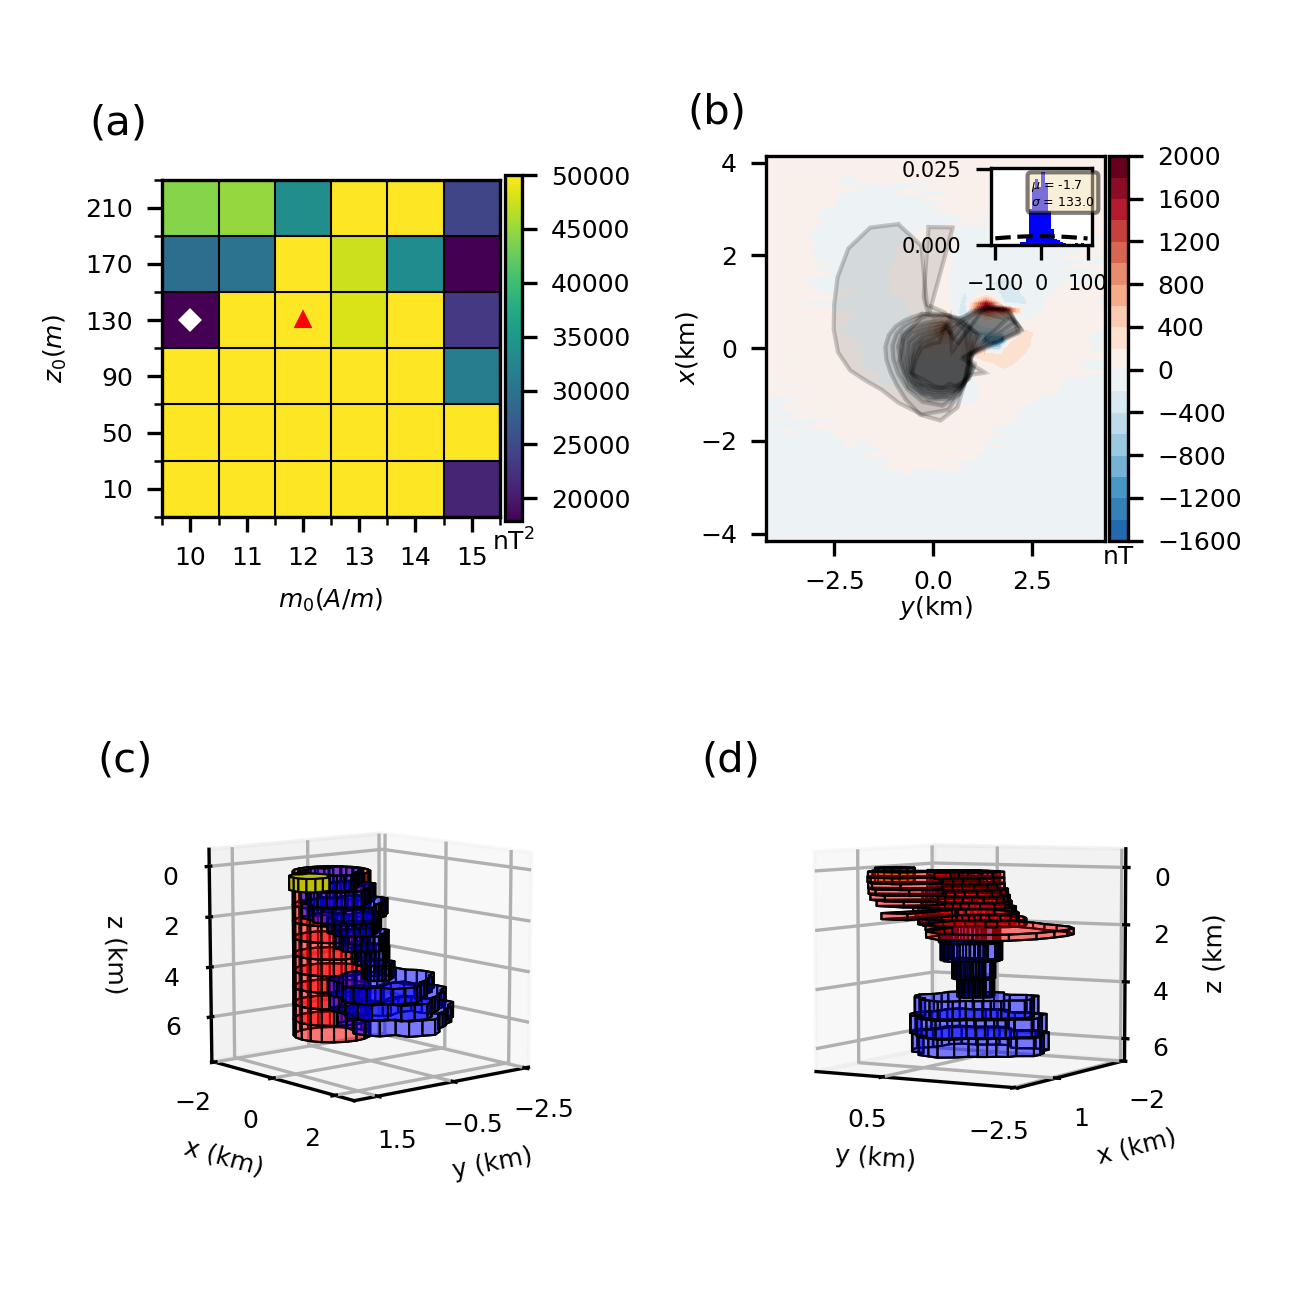
\includegraphics[width=\textwidth]{thick-l2-solution.png}
	\caption{Soluções L2 obtidas para o modelo da fonte alvo com uma fonte interferente grande. 
	(a) Mapa discreto da função objetivo produzida pelos modelos da malha de varredura para valores de profundidade do topo $z_{0}$ e intensidade de magnetização total $m_{0}$. 
	Os valores verdadeiros de $m_{0}$ e $z_{0})$ e aqueles que definem a melhor solução L2 são representados pelo triângulo vermelho e pelo losango branco, respectivamente.
	(b) Resíduos entre os dados contaminados com ruído (Fig. \ref{fig:target_model}a) 
	e os dados preditos (não mostrados) produzidos pela melhor solução L2 (prismas vermelhos no painel d). 
	O histograma dos resíduos inserido em (b) mostra a curva Gaussiana ajustada (curva tracejada).
	Os polígonos cinzas representam as projeções horizontais de todos os prismas que compõe a melhor solução. 
	(c) e (d) Visualização em perspectiva da aproximação inicial (prismas vermelhos) e 
	a melhor solução (prismas vermelhos), respectivamente. Os prismas azuis são o modelo da fonte alvo. 
	}
	\label{fig:thick_l2_result}
\end{figure}

\begin{figure}[!htb]
	\centering
	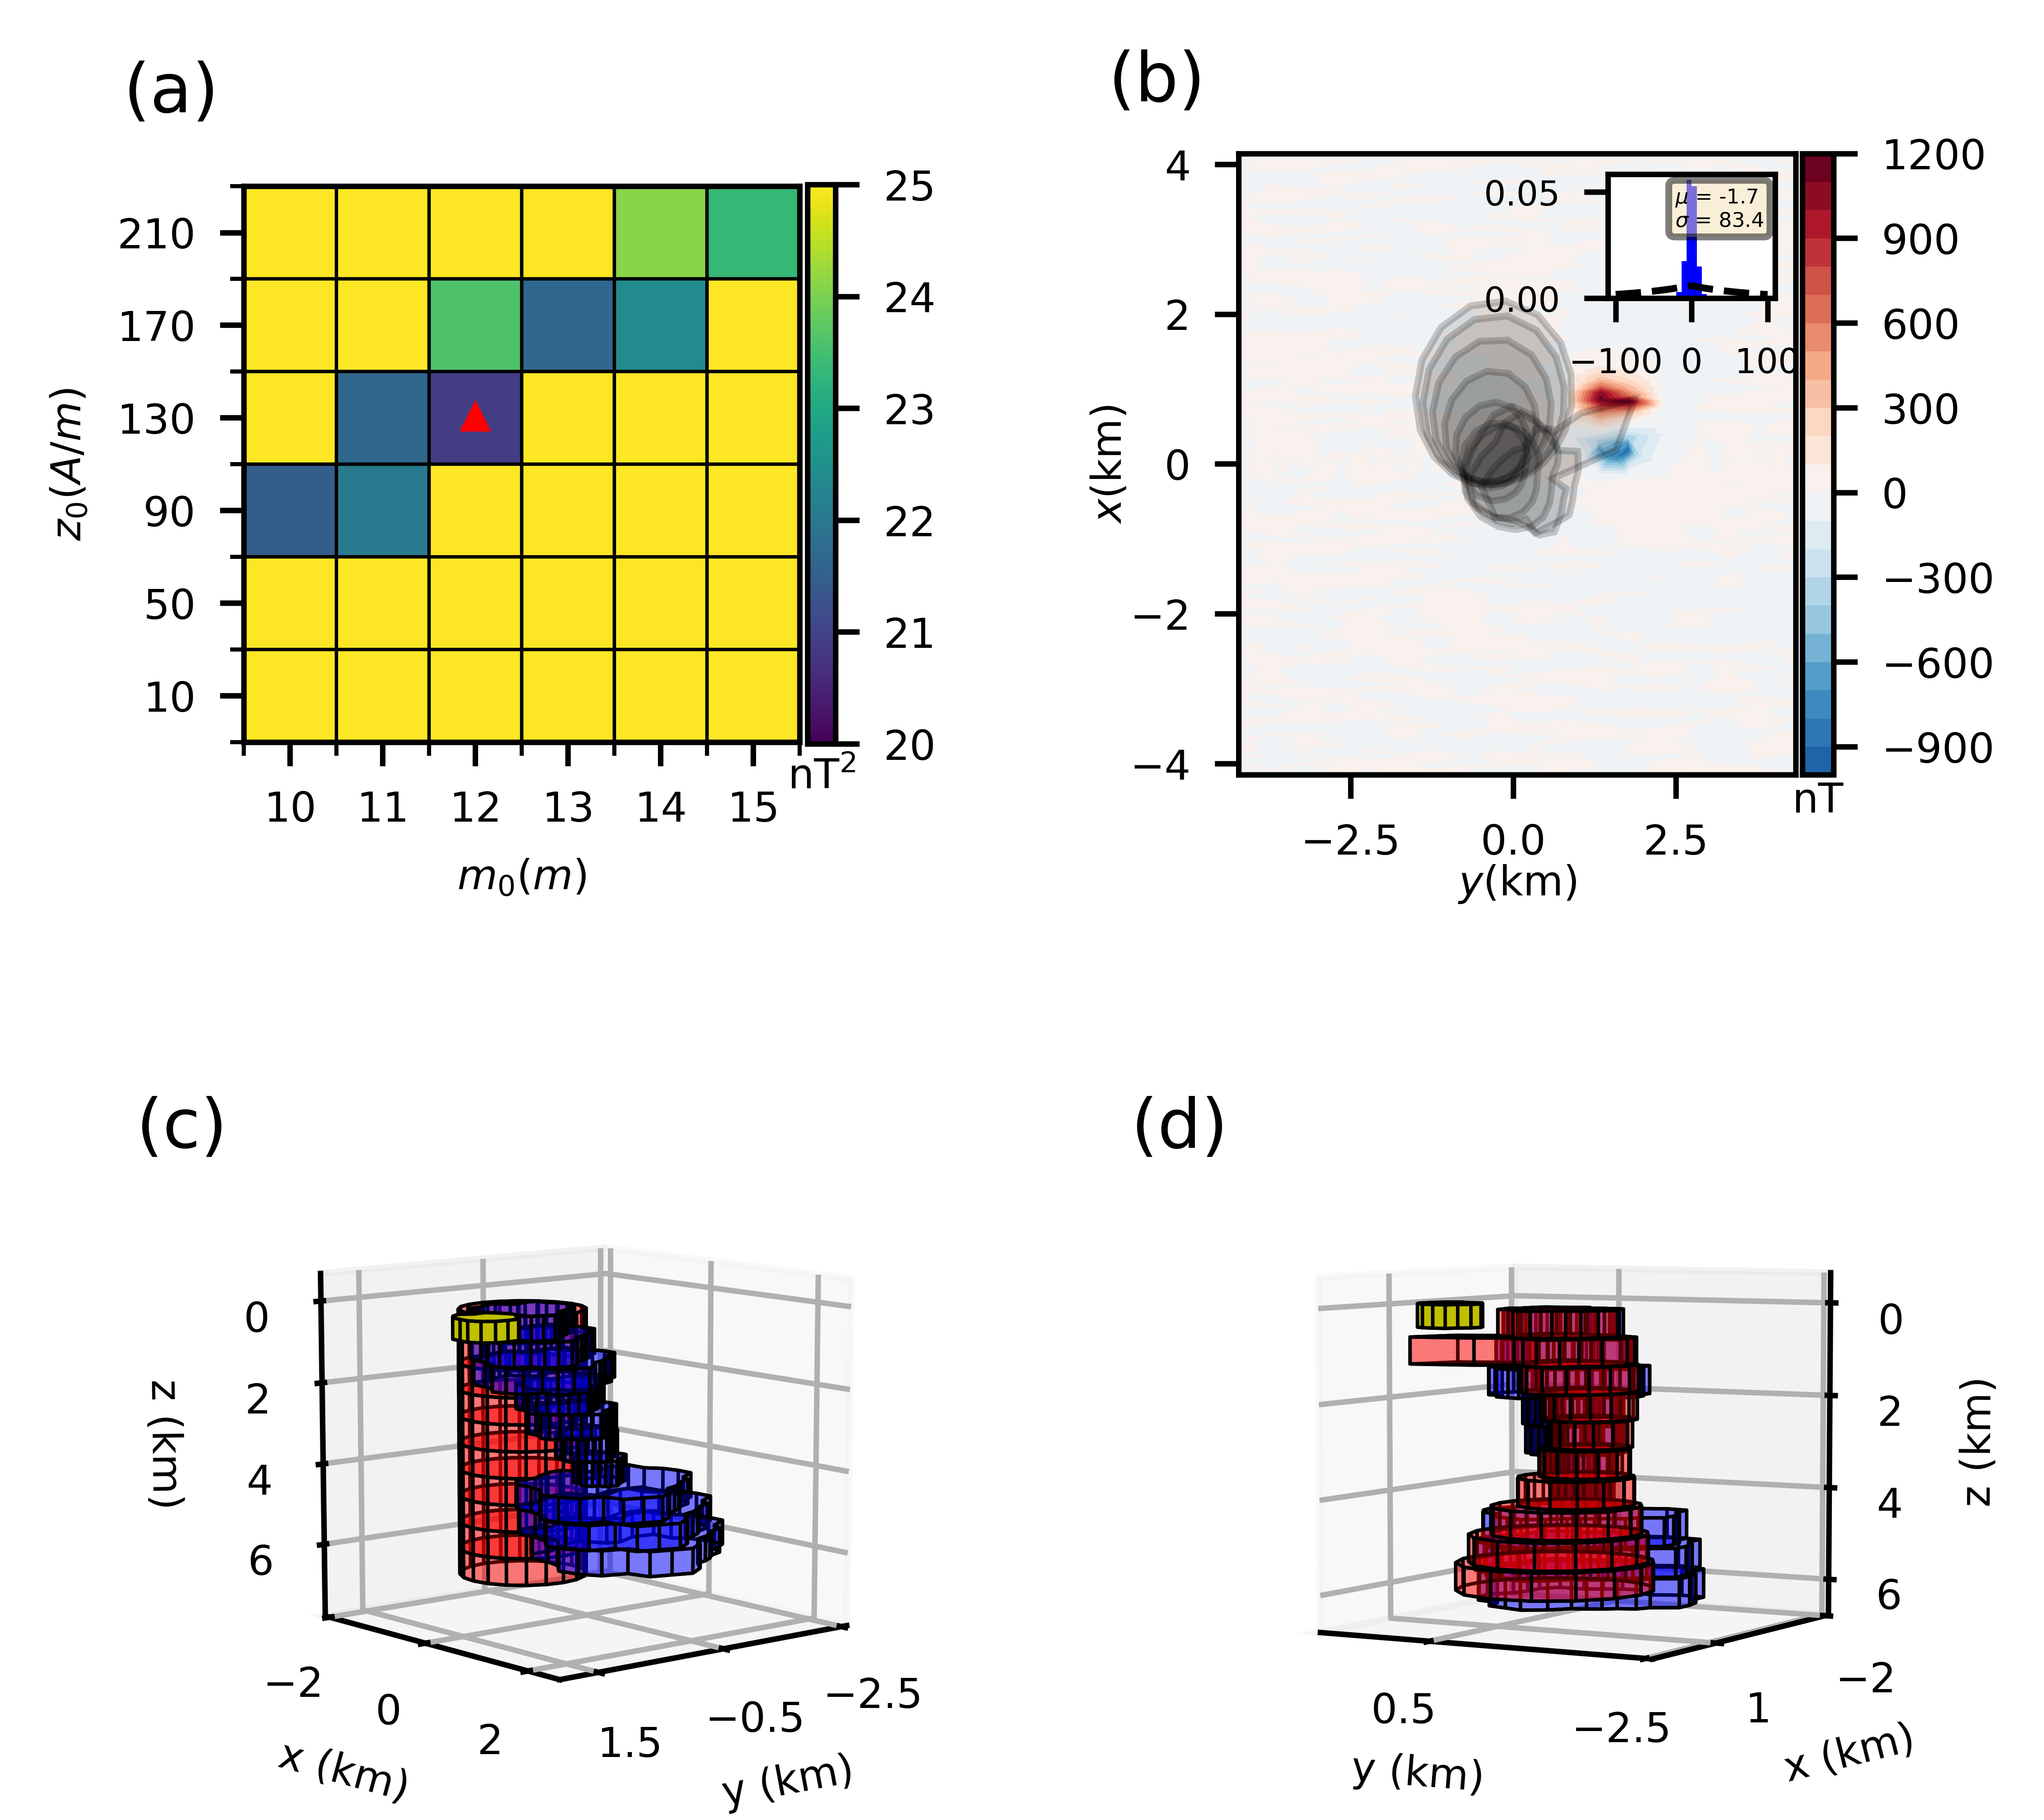
\includegraphics[width=\textwidth]{thick-l1-solution.png}
	\caption{Soluções L1 obtidas para o modelo da fonte alvo com uma fonte interferente grande. 
		(a) Mapa discreto da função objetivo produzida pelos modelos da malha de varredura para valores de profundidade do topo $z_{0}$ e intensidade de magnetização total $m_{0}$. 
		Ambos valores verdadeiros de $m_{0}$ e $z_{0})$ e aqueles que definem a melhor solução L1 são representados pelo triângulo vermelho.
		(b) Resíduos entre os dados contaminados com ruído (Fig. \ref{fig:target_model}a) 
		e os dados preditos (não mostrados) produzidos pela melhor solução L1 (prismas vermelhos no painel d). 
		O histograma dos resíduos inserido em (b) mostra a curva Gaussiana ajustada (curva tracejada).
		Os polígonos cinzas representam as projeções horizontais de todos os prismas que compõe a melhor solução. 
		(c) e (d) Visualização em perspectiva da aproximação inicial (prismas vermelhos) e 
		a melhor solução (prismas vermelhos), respectivamente. Os prismas azuis são o modelo da fonte alvo. 
	}
	\label{fig:thick_l1_result}
\end{figure}